% Options for packages loaded elsewhere
\PassOptionsToPackage{unicode}{hyperref}
\PassOptionsToPackage{hyphens}{url}
%
\documentclass[
]{article}
\title{SI Figures for \emph{Codistribution as an indicator of whole
metacommunity response to environmental change.}}
\author{Authorship Redacted for blind review}
\date{}

\usepackage{amsmath,amssymb}
\usepackage{lmodern}
\usepackage{iftex}
\ifPDFTeX
  \usepackage[T1]{fontenc}
  \usepackage[utf8]{inputenc}
  \usepackage{textcomp} % provide euro and other symbols
\else % if luatex or xetex
  \usepackage{unicode-math}
  \defaultfontfeatures{Scale=MatchLowercase}
  \defaultfontfeatures[\rmfamily]{Ligatures=TeX,Scale=1}
\fi
% Use upquote if available, for straight quotes in verbatim environments
\IfFileExists{upquote.sty}{\usepackage{upquote}}{}
\IfFileExists{microtype.sty}{% use microtype if available
  \usepackage[]{microtype}
  \UseMicrotypeSet[protrusion]{basicmath} % disable protrusion for tt fonts
}{}
\makeatletter
\@ifundefined{KOMAClassName}{% if non-KOMA class
  \IfFileExists{parskip.sty}{%
    \usepackage{parskip}
  }{% else
    \setlength{\parindent}{0pt}
    \setlength{\parskip}{6pt plus 2pt minus 1pt}}
}{% if KOMA class
  \KOMAoptions{parskip=half}}
\makeatother
\usepackage{xcolor}
\IfFileExists{xurl.sty}{\usepackage{xurl}}{} % add URL line breaks if available
\IfFileExists{bookmark.sty}{\usepackage{bookmark}}{\usepackage{hyperref}}
\hypersetup{
  pdftitle={SI Figures for Codistribution as an indicator of whole metacommunity response to environmental change.},
  pdfauthor={Authorship Redacted for blind review},
  hidelinks,
  pdfcreator={LaTeX via pandoc}}
\urlstyle{same} % disable monospaced font for URLs
\usepackage[margin=1in]{geometry}
\usepackage{longtable,booktabs,array}
\usepackage{calc} % for calculating minipage widths
% Correct order of tables after \paragraph or \subparagraph
\usepackage{etoolbox}
\makeatletter
\patchcmd\longtable{\par}{\if@noskipsec\mbox{}\fi\par}{}{}
\makeatother
% Allow footnotes in longtable head/foot
\IfFileExists{footnotehyper.sty}{\usepackage{footnotehyper}}{\usepackage{footnote}}
\makesavenoteenv{longtable}
\usepackage{graphicx}
\makeatletter
\def\maxwidth{\ifdim\Gin@nat@width>\linewidth\linewidth\else\Gin@nat@width\fi}
\def\maxheight{\ifdim\Gin@nat@height>\textheight\textheight\else\Gin@nat@height\fi}
\makeatother
% Scale images if necessary, so that they will not overflow the page
% margins by default, and it is still possible to overwrite the defaults
% using explicit options in \includegraphics[width, height, ...]{}
\setkeys{Gin}{width=\maxwidth,height=\maxheight,keepaspectratio}
% Set default figure placement to htbp
\makeatletter
\def\fps@figure{htbp}
\makeatother
\setlength{\emergencystretch}{3em} % prevent overfull lines
\providecommand{\tightlist}{%
  \setlength{\itemsep}{0pt}\setlength{\parskip}{0pt}}
\setcounter{secnumdepth}{-\maxdimen} % remove section numbering
\usepackage{float} \floatplacement{figure}{H}
\ifLuaTeX
  \usepackage{selnolig}  % disable illegal ligatures
\fi

\begin{document}
\maketitle

{
\setcounter{tocdepth}{2}
\tableofcontents
}
\newpage

\hypertarget{simulations}{%
\section{Simulations}\label{simulations}}

\hypertarget{simulation-setup-example}{%
\subsection{Simulation Setup Example}\label{simulation-setup-example}}

\begin{figure}
\centering
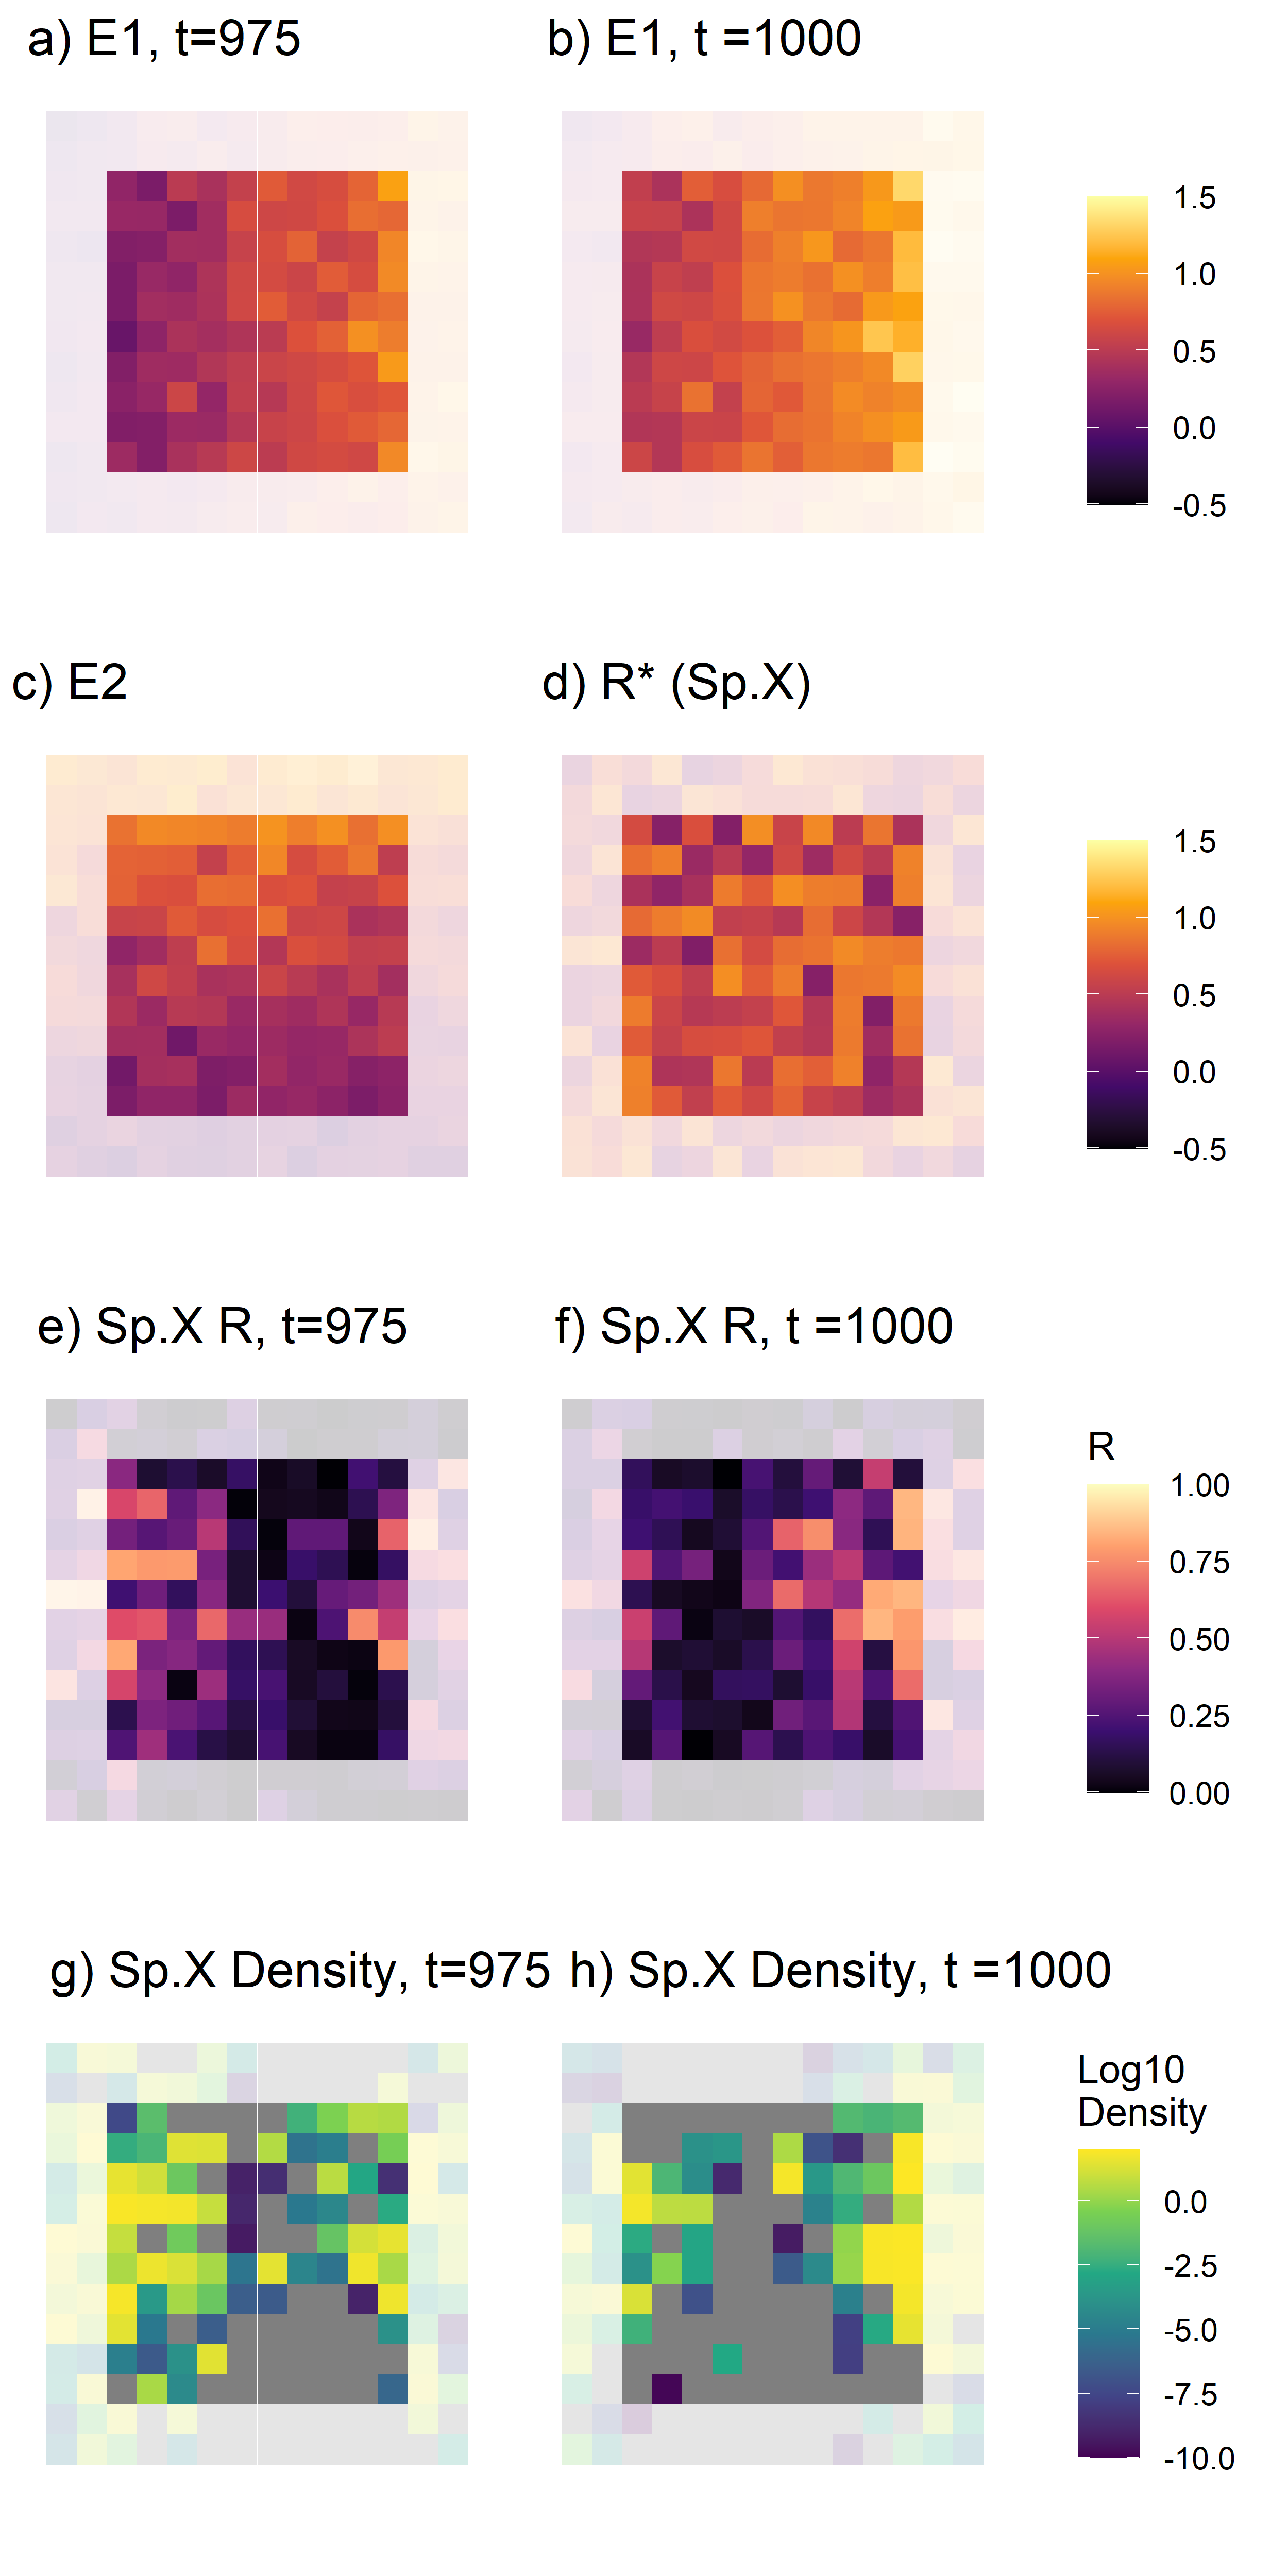
\includegraphics[width=\textwidth,height=0.65\textheight]{SimulationMarkdowns/Figures/SimulationExample_grid.png}
\caption{Example illustration of the simulation model, focussing on an
single species. Values are drawn from the same simulation as illustrated
in the main text Figure 2. Values from the peripheral sites not used for
the JSDM fitting are shown greyed out. a) Pre-change distribution of
\(E_1\) variable. This variable increases through time, and could be
considered `temperature'. b) \(E_1\) variable at \(t=1000\).
c)Distribution of \(E_2\). This variable is fixed throughout the
simulation and so could be considered an aspect of geology. d)
Distribution of \(E_3\) for the example focal species. This variable
adds additional fixed heterogeneity in growth rates distinct for each
species to the simulation. e) Growth rate \(R\), of an example species
before the onset of climate change. Note the approximately circular
shape, but the high degree of heterogeneity. f) Growth rate \(R\) of the
example species after 25 time steps of climate change (\(t=1000\)). Note
the leftwards shift in the optimal (bright colours) habitat. g)
Pre-climate change distribution of an example species. Note the
approximate correspondence with the growth rates, but also infilling due
to dispersal mass-effects h) Mid-climate change distribution of the
example species. Note the movement lags - the shift leftwards movement
is not as noticeable as in the growth rates (f).}
\end{figure}

\hypertarget{impact-of-parameters-on-metacommunity-size-and-occupancy}{%
\subsection{Impact of parameters on metacommunity size and
occupancy}\label{impact-of-parameters-on-metacommunity-size-and-occupancy}}

\begin{figure}
\centering
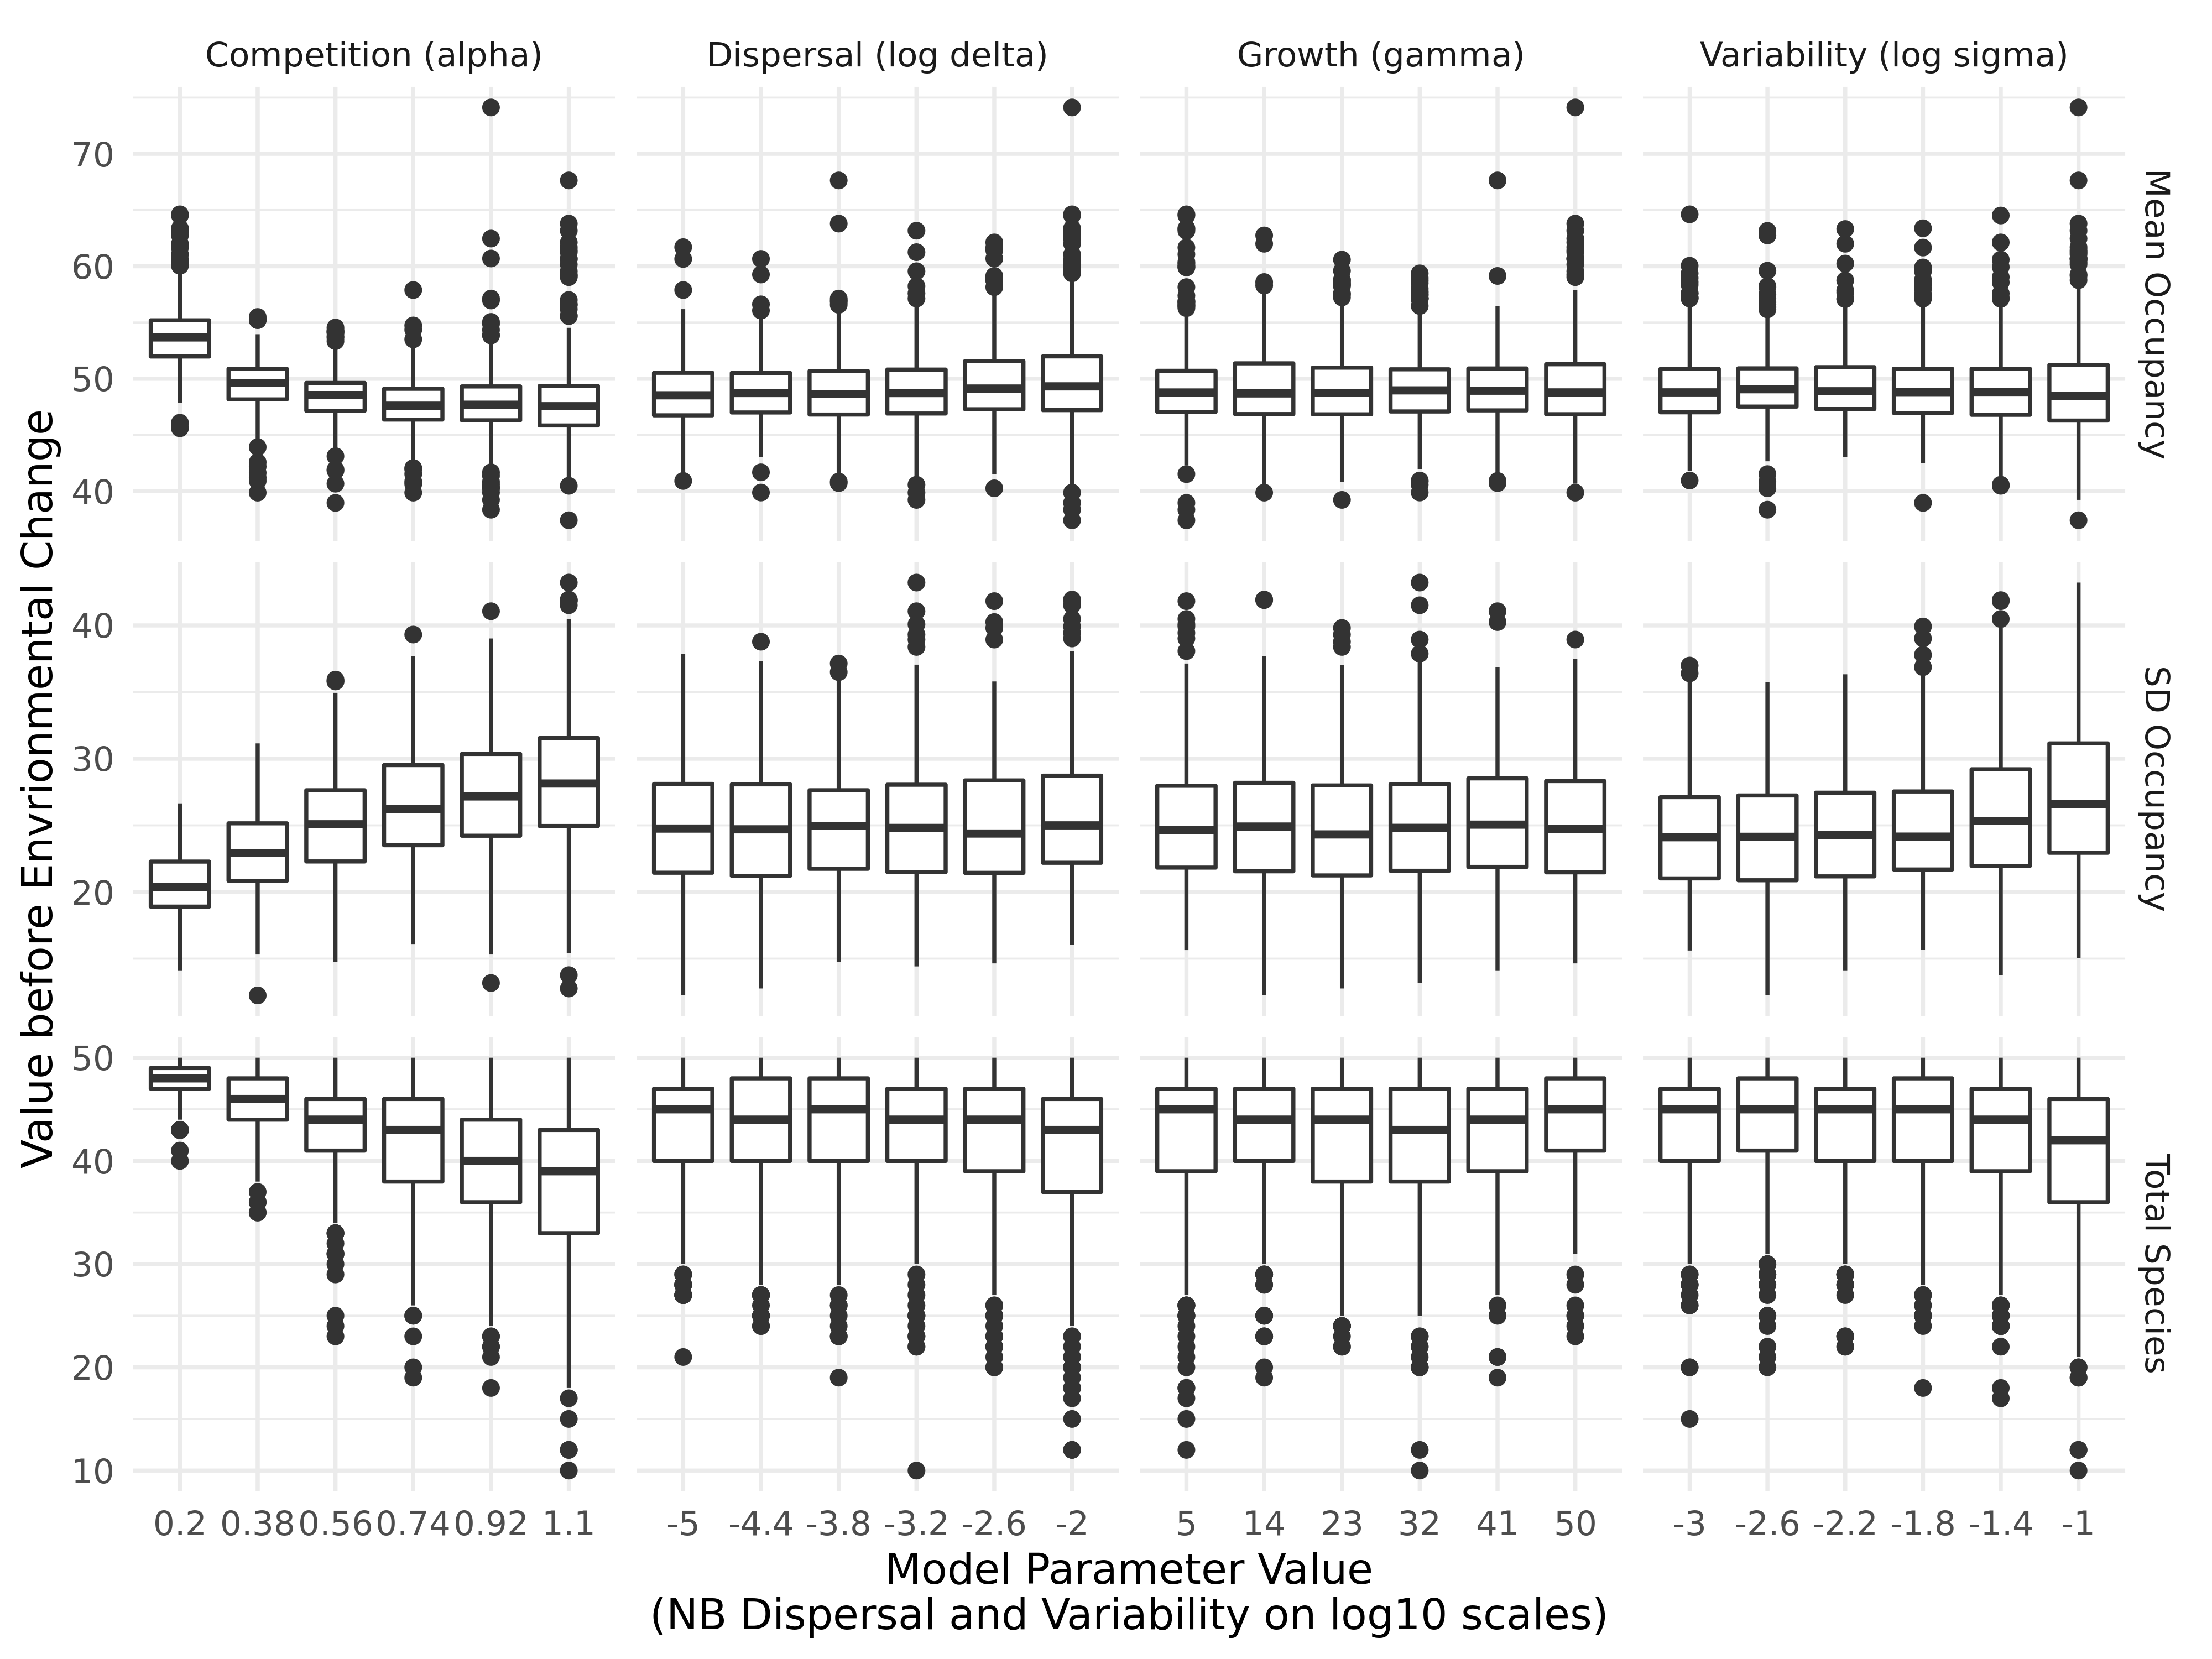
\includegraphics{SimulationMarkdowns/Figures/OccuBefore.png}
\caption{Impact of simulation model parameters on key metacommunity
statistics prior to the introduction of environmental change. Only
species that are used in the JSDMs are included here, i.e.~excluding
those that are too rare (or abundant) within the focal squares. Each
facet includes all 2460 simulations, but are separated by different
responses and driving parameters. Boxplots hinges show 25 and 75th
percentiles. Note \(log_{10}\) scales used for dispersal and
environmental stochasticity parameters.}
\end{figure}

\hypertarget{impact-of-parameters-on-simulated-metacommunity-structure}{%
\subsection{Impact of parameters on simulated metacommunity
structure}\label{impact-of-parameters-on-simulated-metacommunity-structure}}

\begin{figure}
\centering
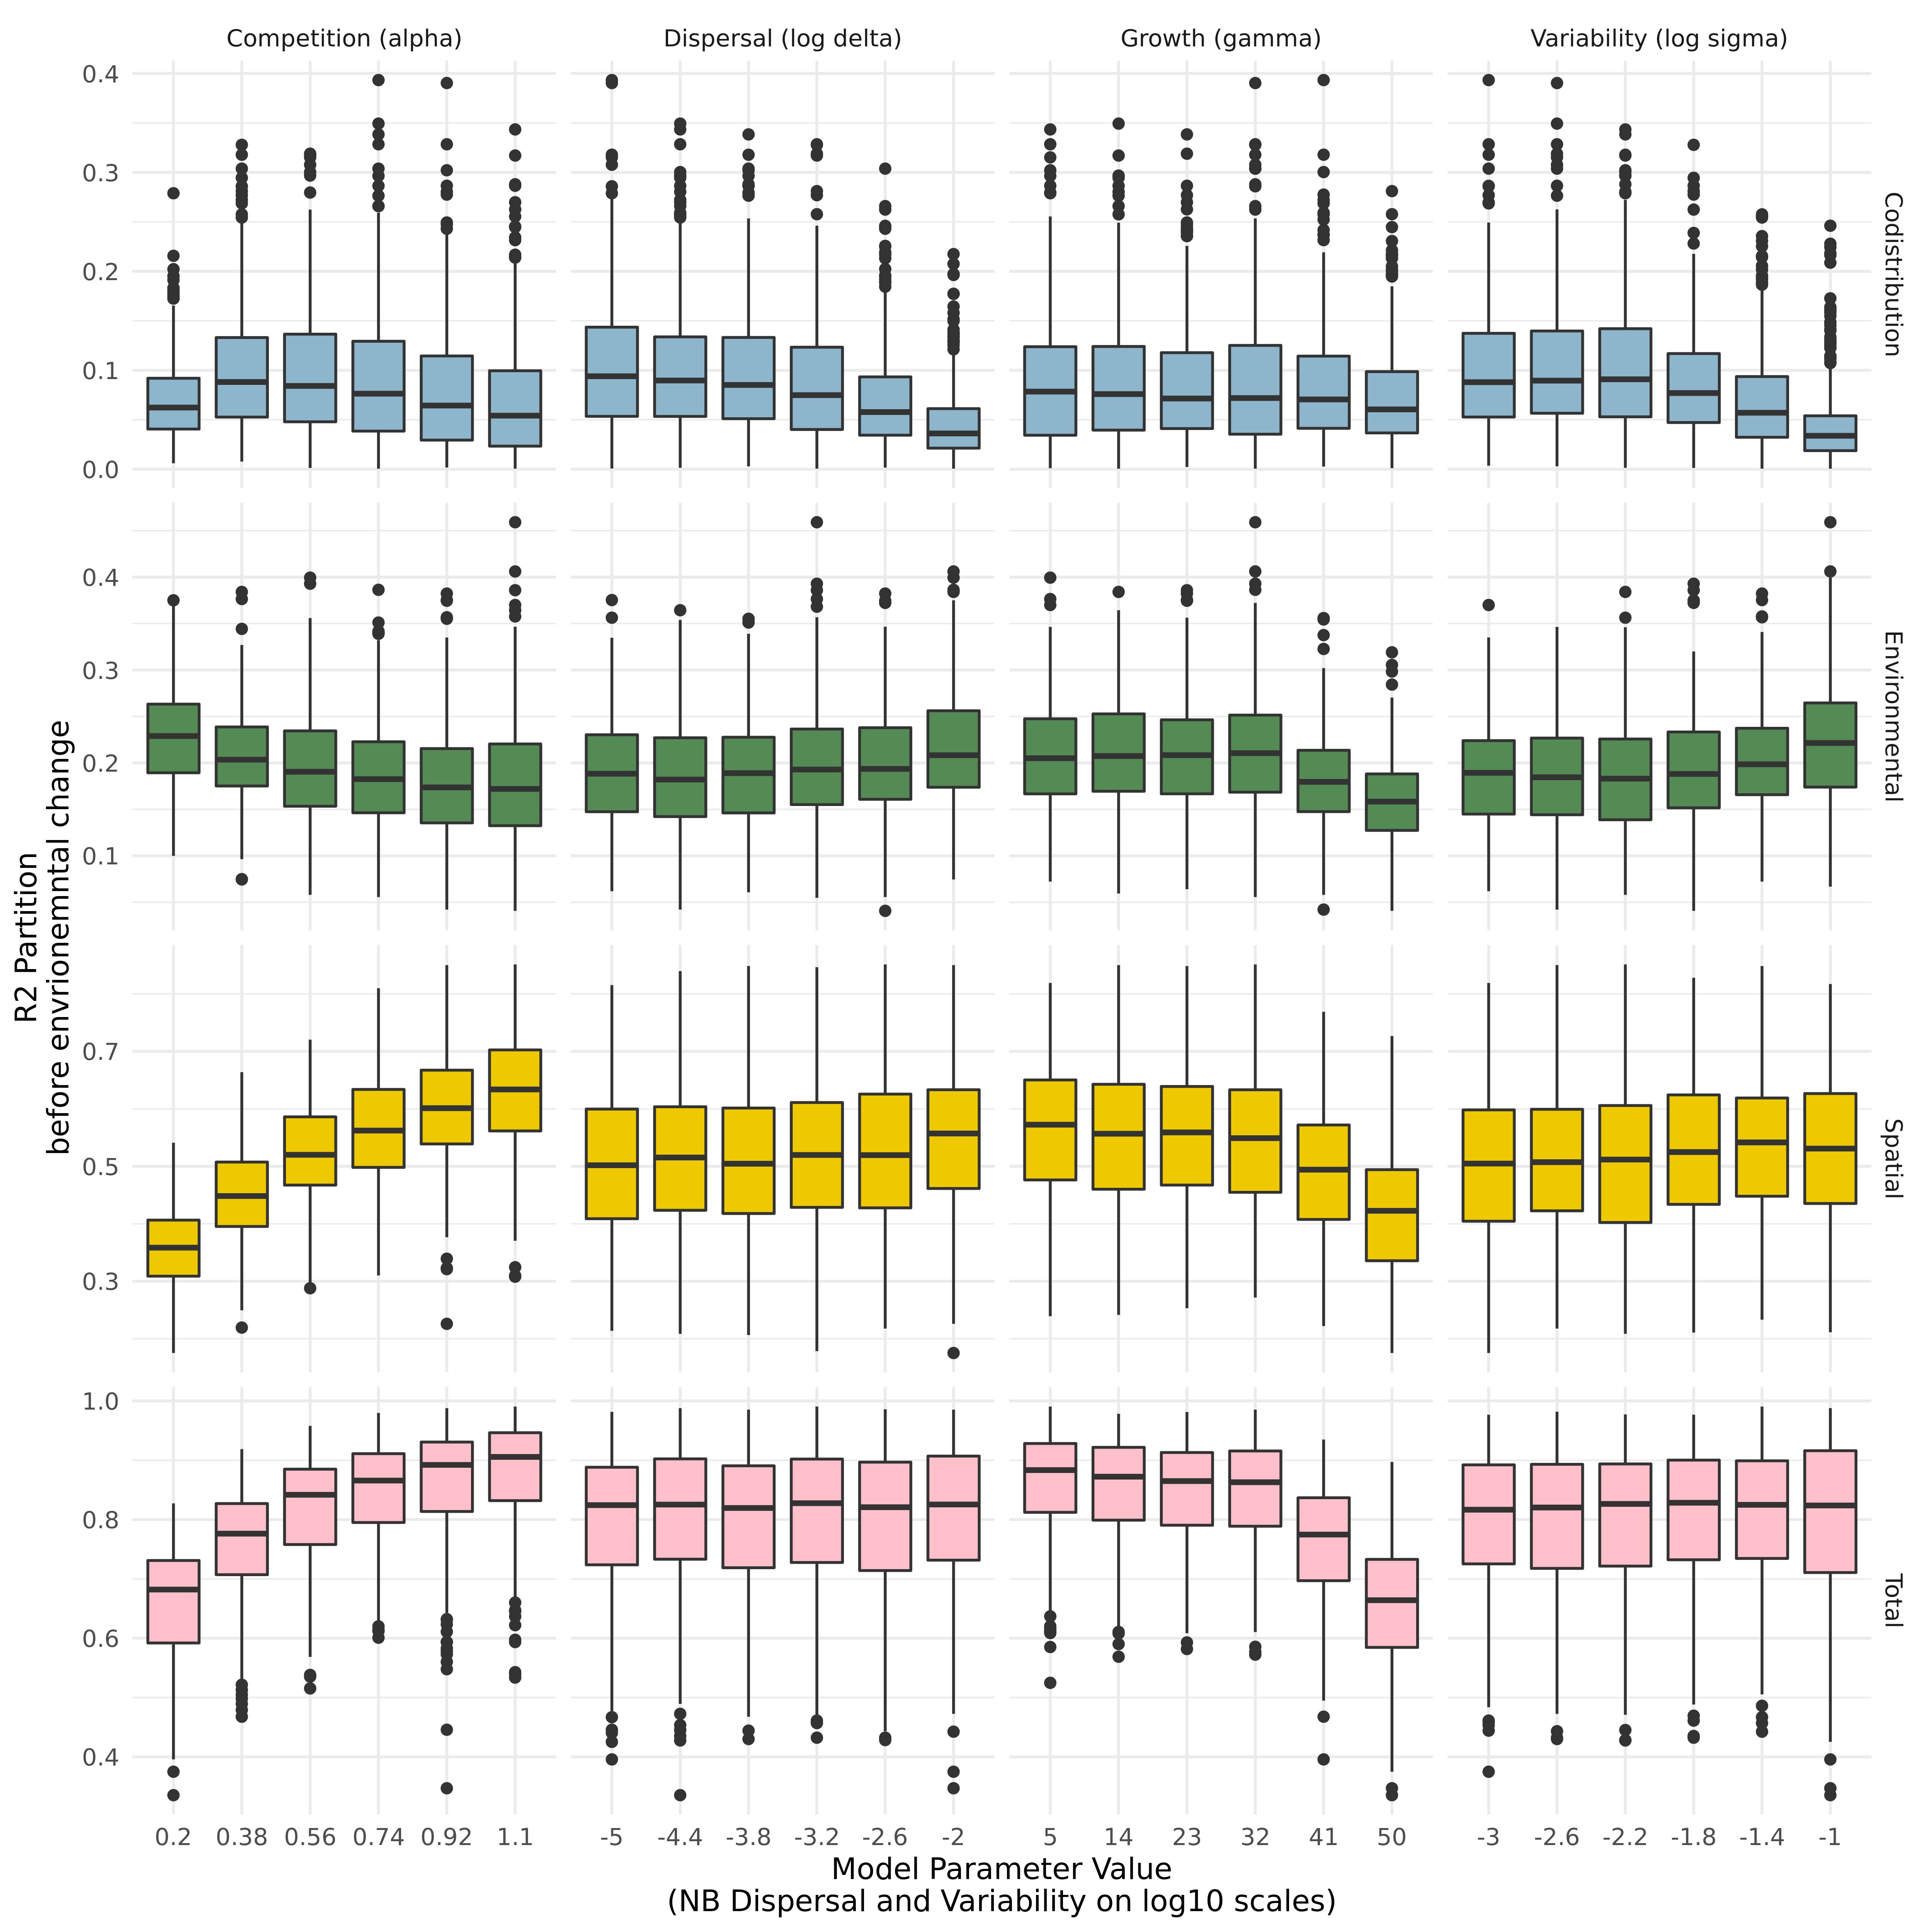
\includegraphics{SimulationMarkdowns/Figures/ParamStart.png}
\caption{Impact of the model parameters on the simulated metacommunity
structure, as assessed by variance partitioning before the introduction
of environmental change. Boxplots hinges show 25 and 75th percentiles.}
\end{figure}

\hypertarget{impact-of-parameters-on-shift-in-simulated-metacommunity-structure}{%
\subsection{Impact of parameters on shift in simulated metacommunity
structure}\label{impact-of-parameters-on-shift-in-simulated-metacommunity-structure}}

\begin{figure}
\centering
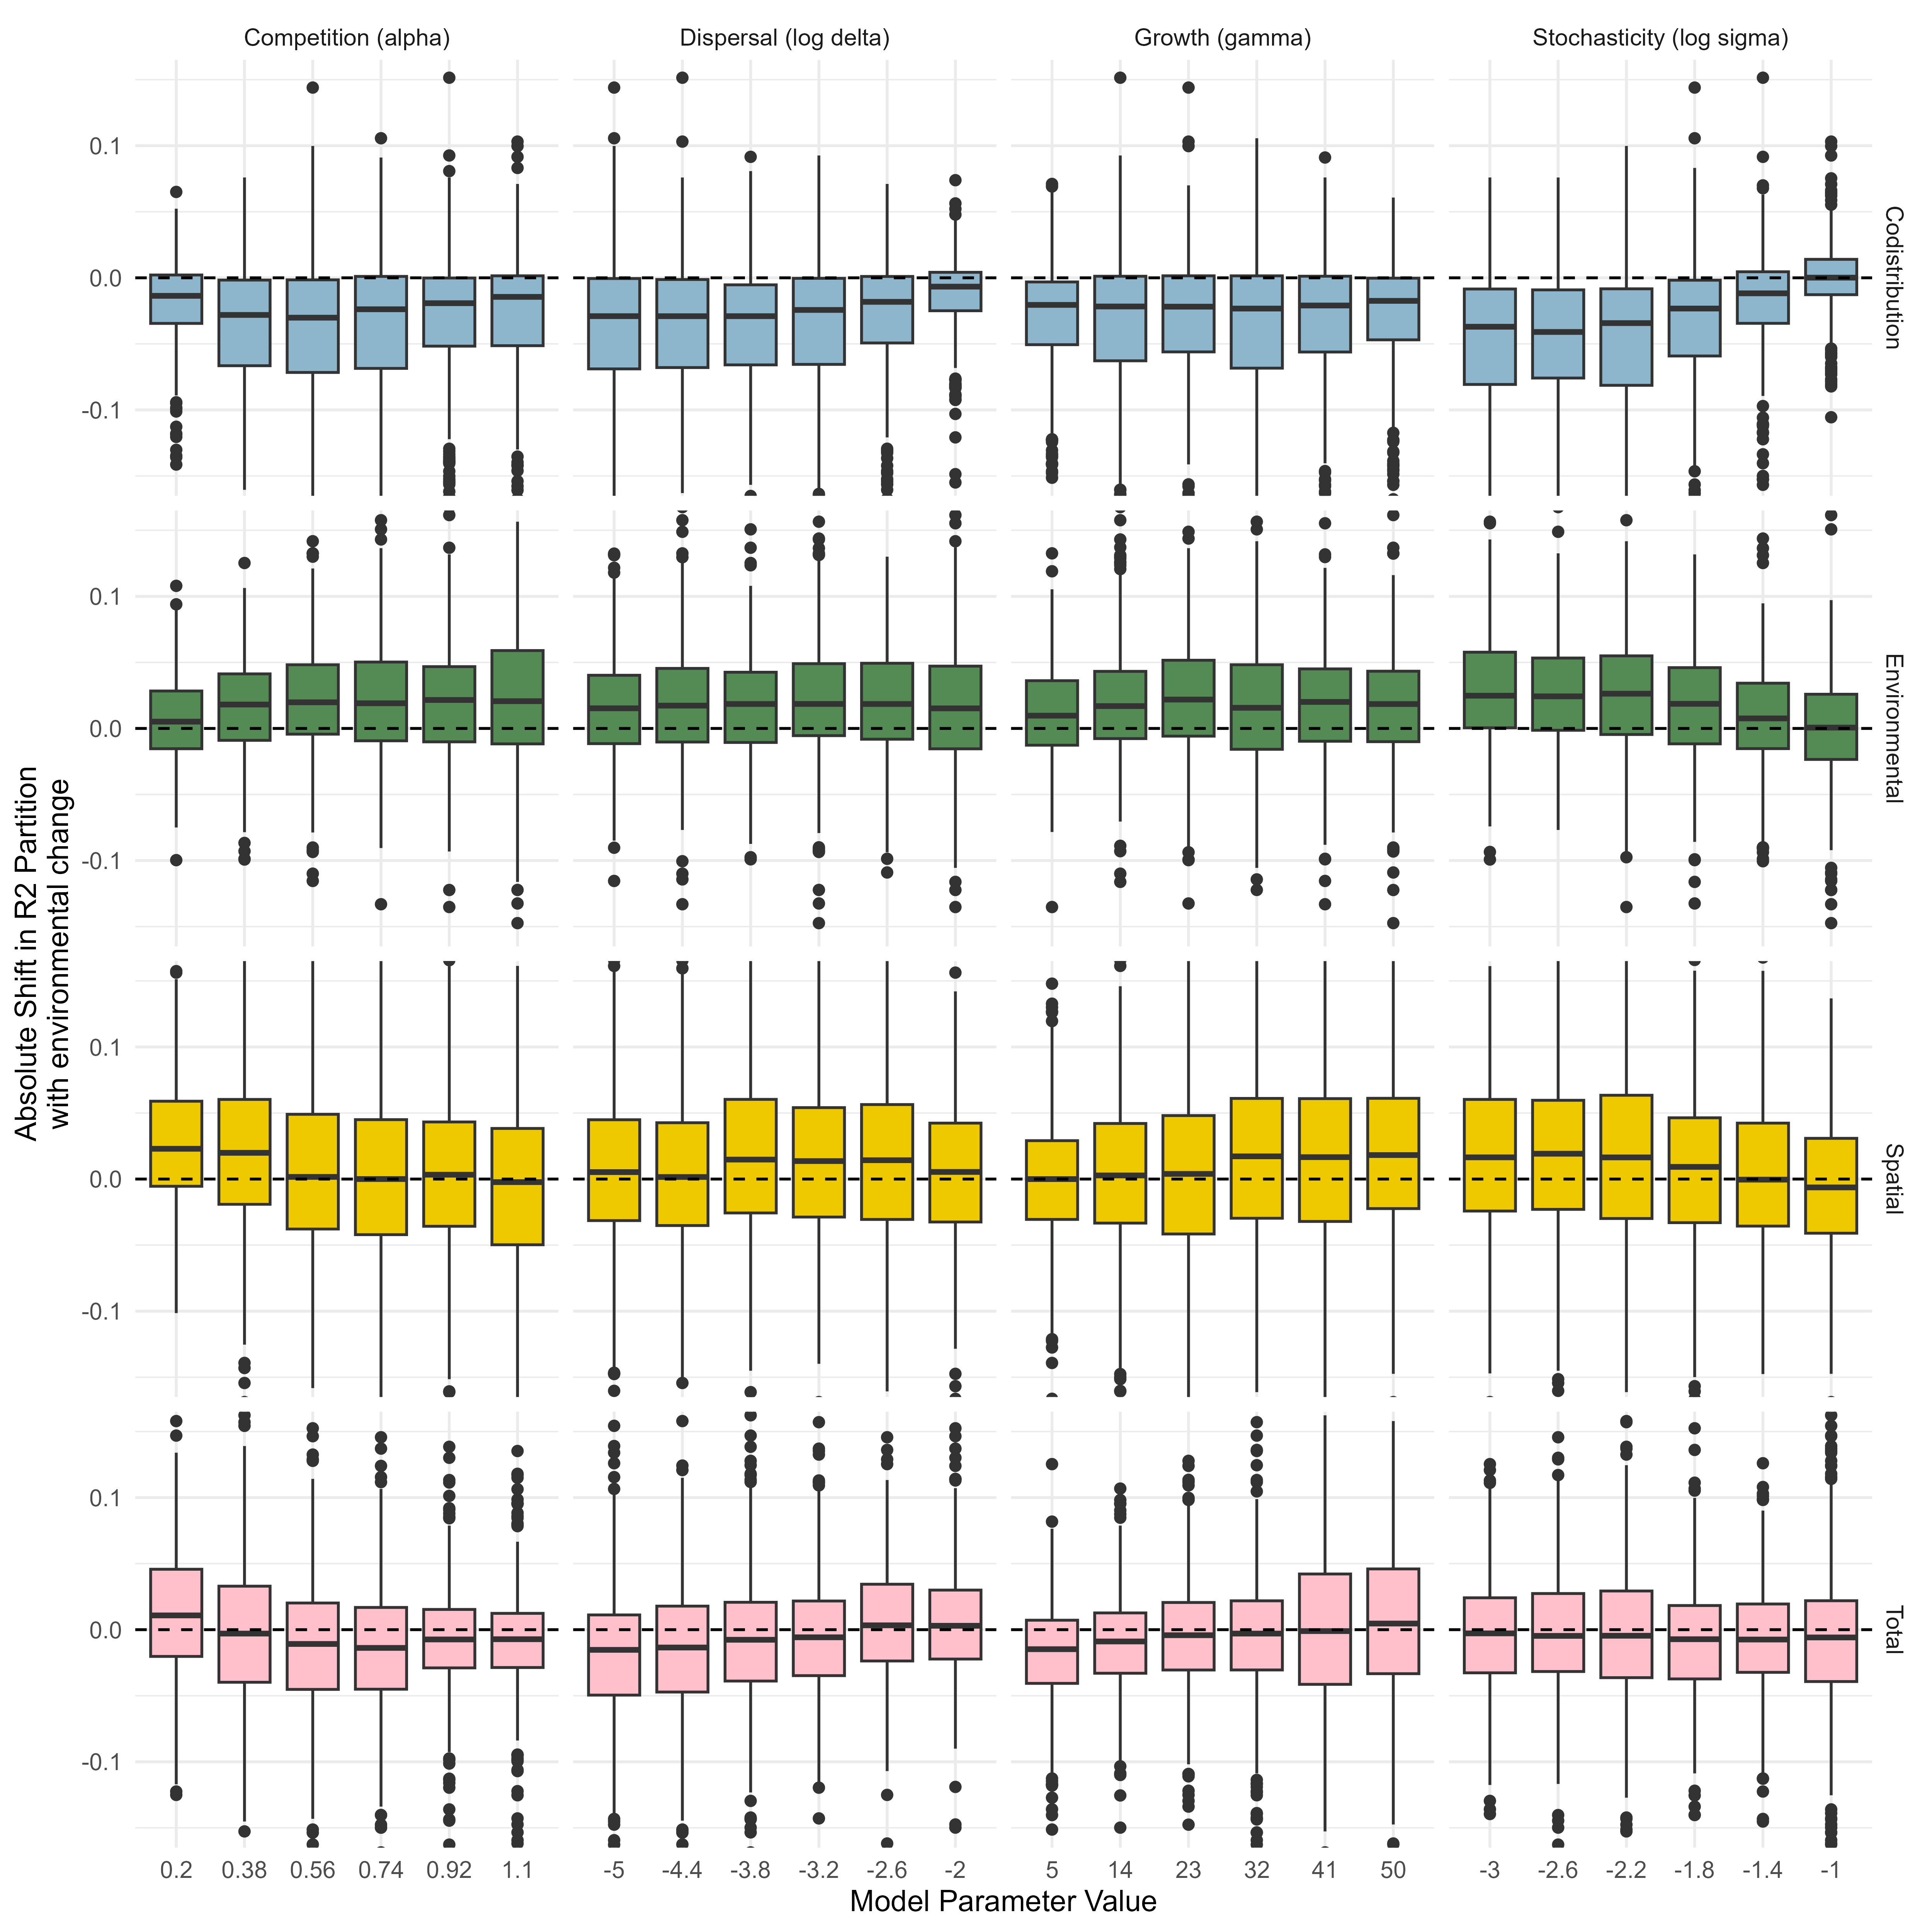
\includegraphics{SimulationMarkdowns/Figures/ParamShift.png}
\caption{The dependence of shifts in the variance partitioning on the
parameters of the simulated metacommunities. Figure 3 in the main text
is a summary of this plot. Boxplots hinges show 25 and 75th
percentiles.}
\end{figure}

\hypertarget{impact-of-false-absences-on-detectability-of-shift-in-metacommunity-structure}{%
\subsection{Impact of false absences on detectability of shift in
metacommunity
structure}\label{impact-of-false-absences-on-detectability-of-shift-in-metacommunity-structure}}

\begin{figure}
\centering
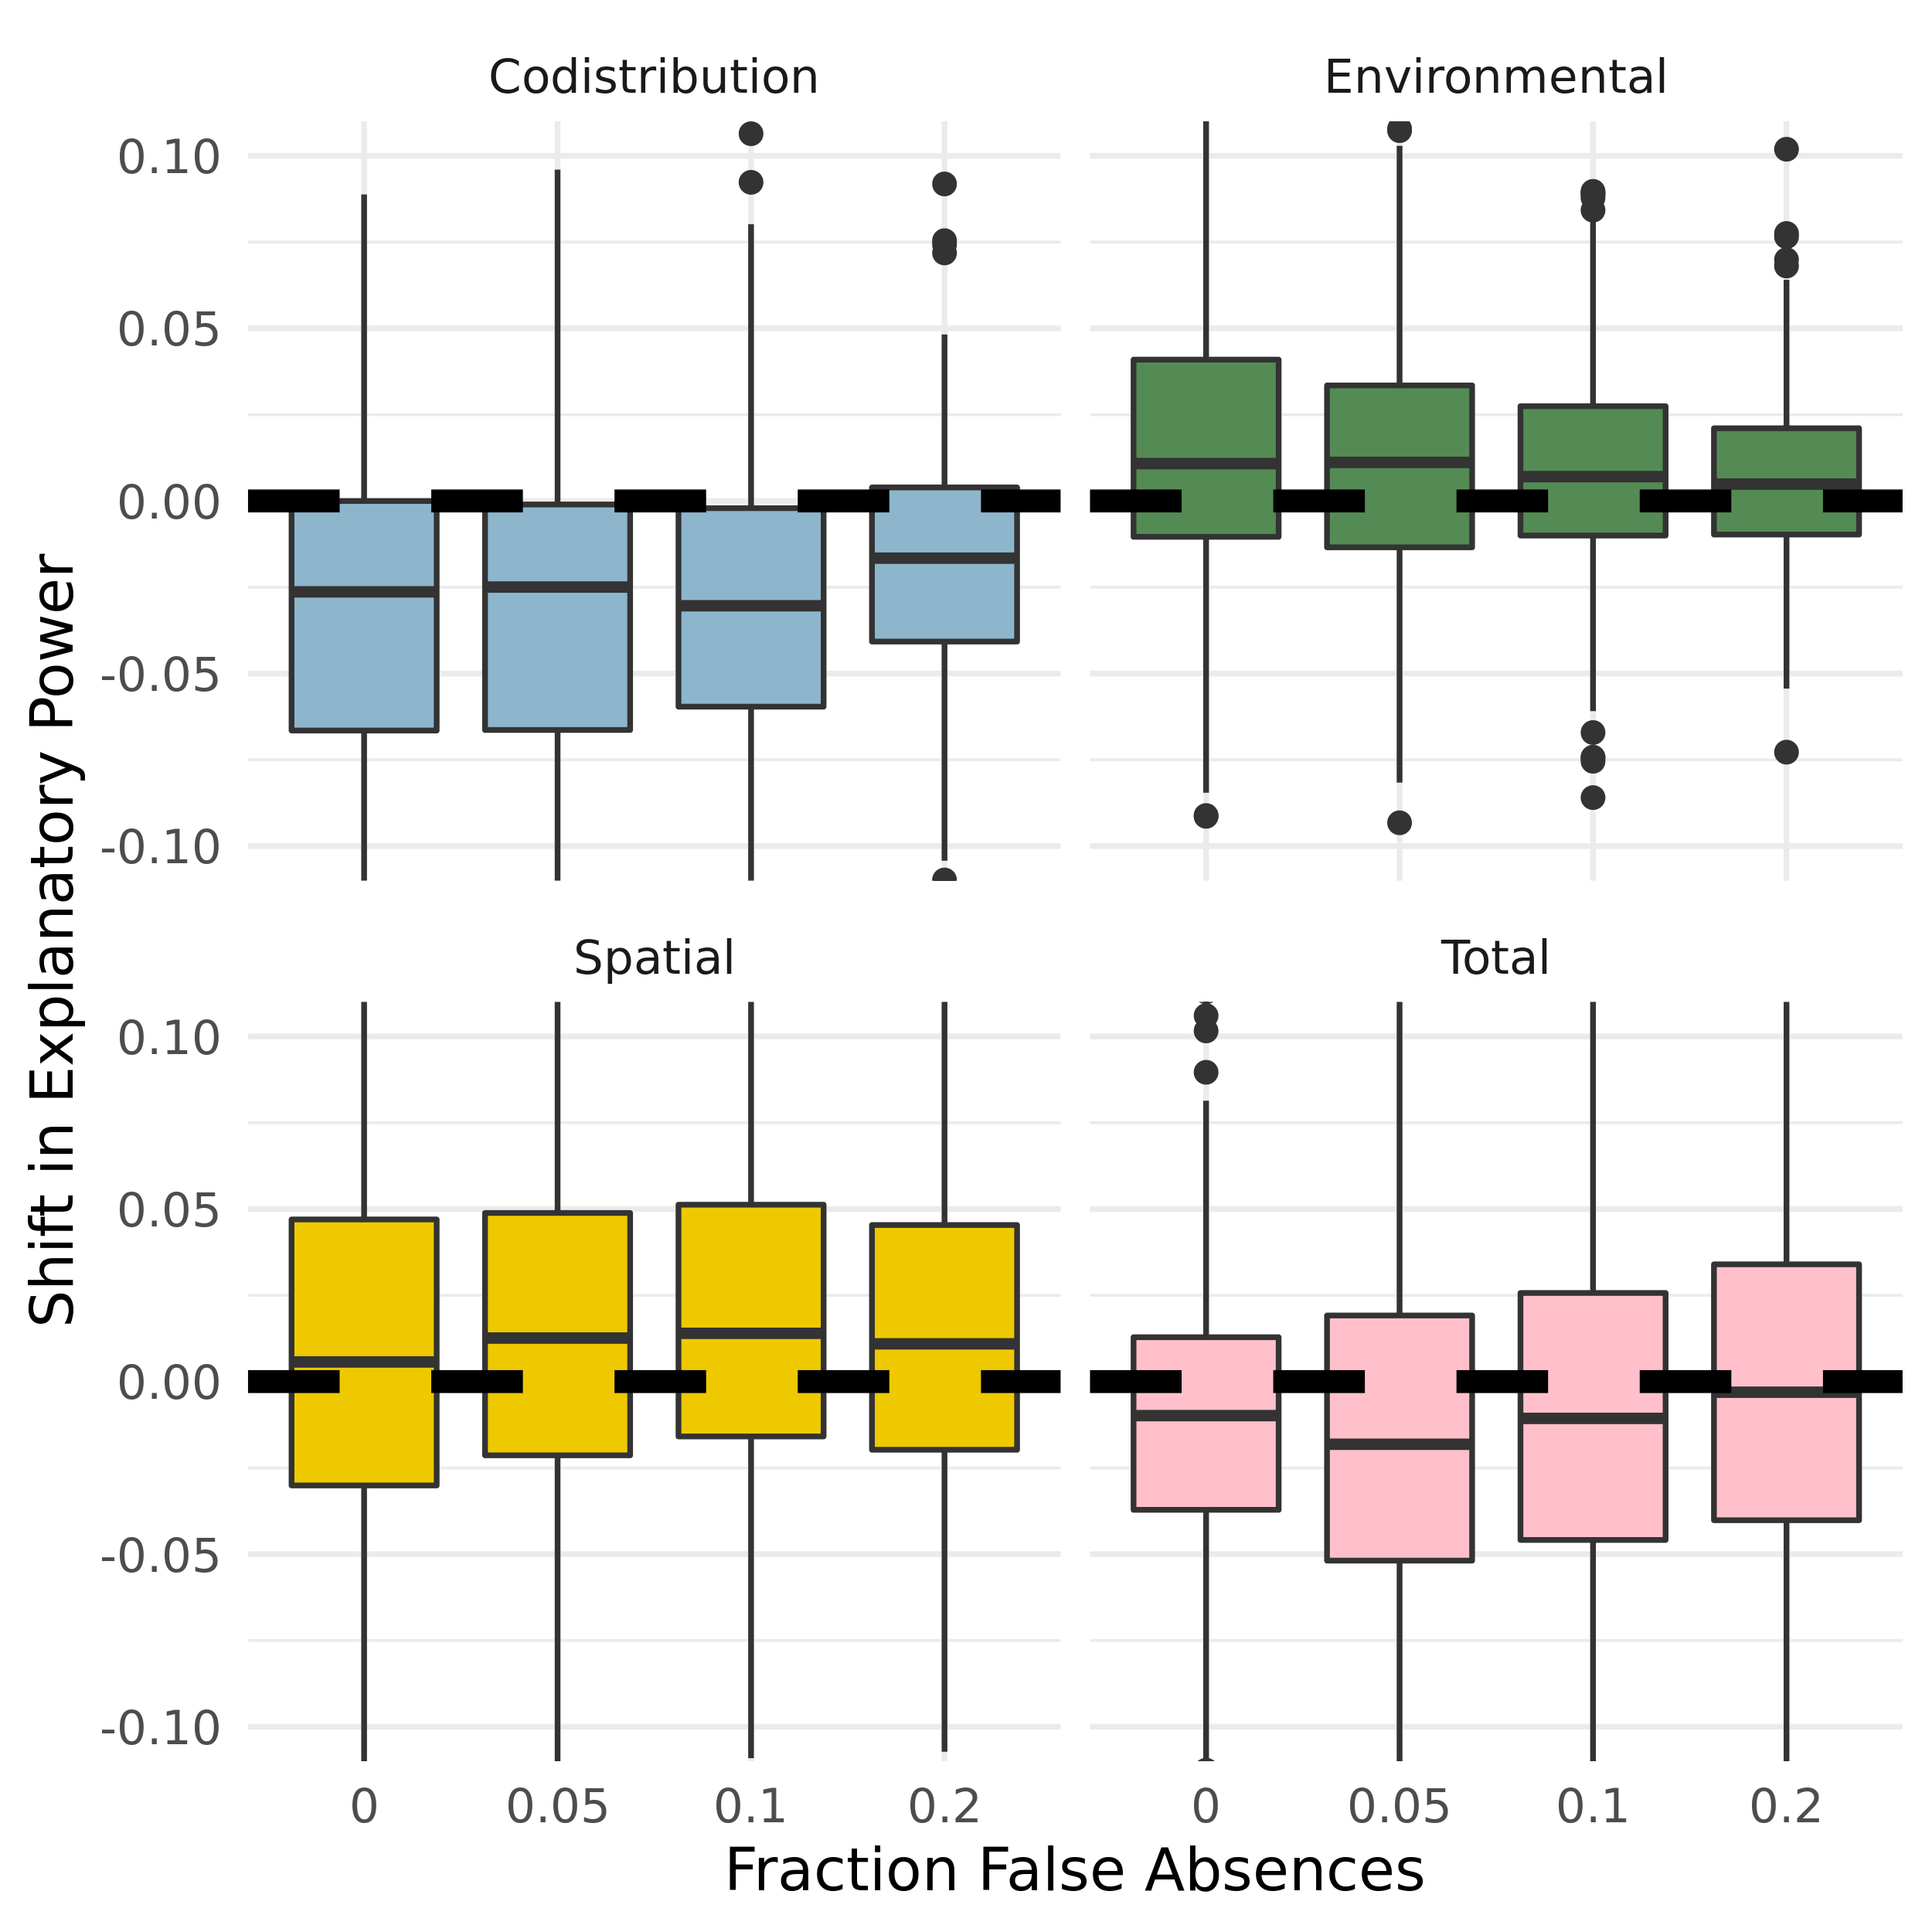
\includegraphics{SimulationMarkdowns/Figures/FalseAbs.png}
\caption{Impact of false absences on the consistent identity of trends.
Simulation was run as with the analysis in the main text, but with a
reduced spread of core model parameters (\(\delta\):
\(10^{-5}, 10^{-4}, 10^{-3}\); \(\alpha\); \(0.3, 0.8, 1.1\),
\(\gamma\): \(5, 20, 40\), \(\sigma\): \(10^{-3}, 10^{-2}, 10^{-1}\)),
crossed with 4 levels of false absences (\(0, 0.05, 0.1, 0.2\)). False
absences are introduced by randomly, and independently, switching each
presence (i.e.~above threshold) to an absence with a given probability.
Boxplots hinges show 25 and 75th percentiles.}
\end{figure}

\hypertarget{butterfly-dataset}{%
\section{Butterfly Dataset}\label{butterfly-dataset}}

\hypertarget{distribution-of-sites}{%
\subsection{Distribution of Sites}\label{distribution-of-sites}}

\begin{figure}
\centering
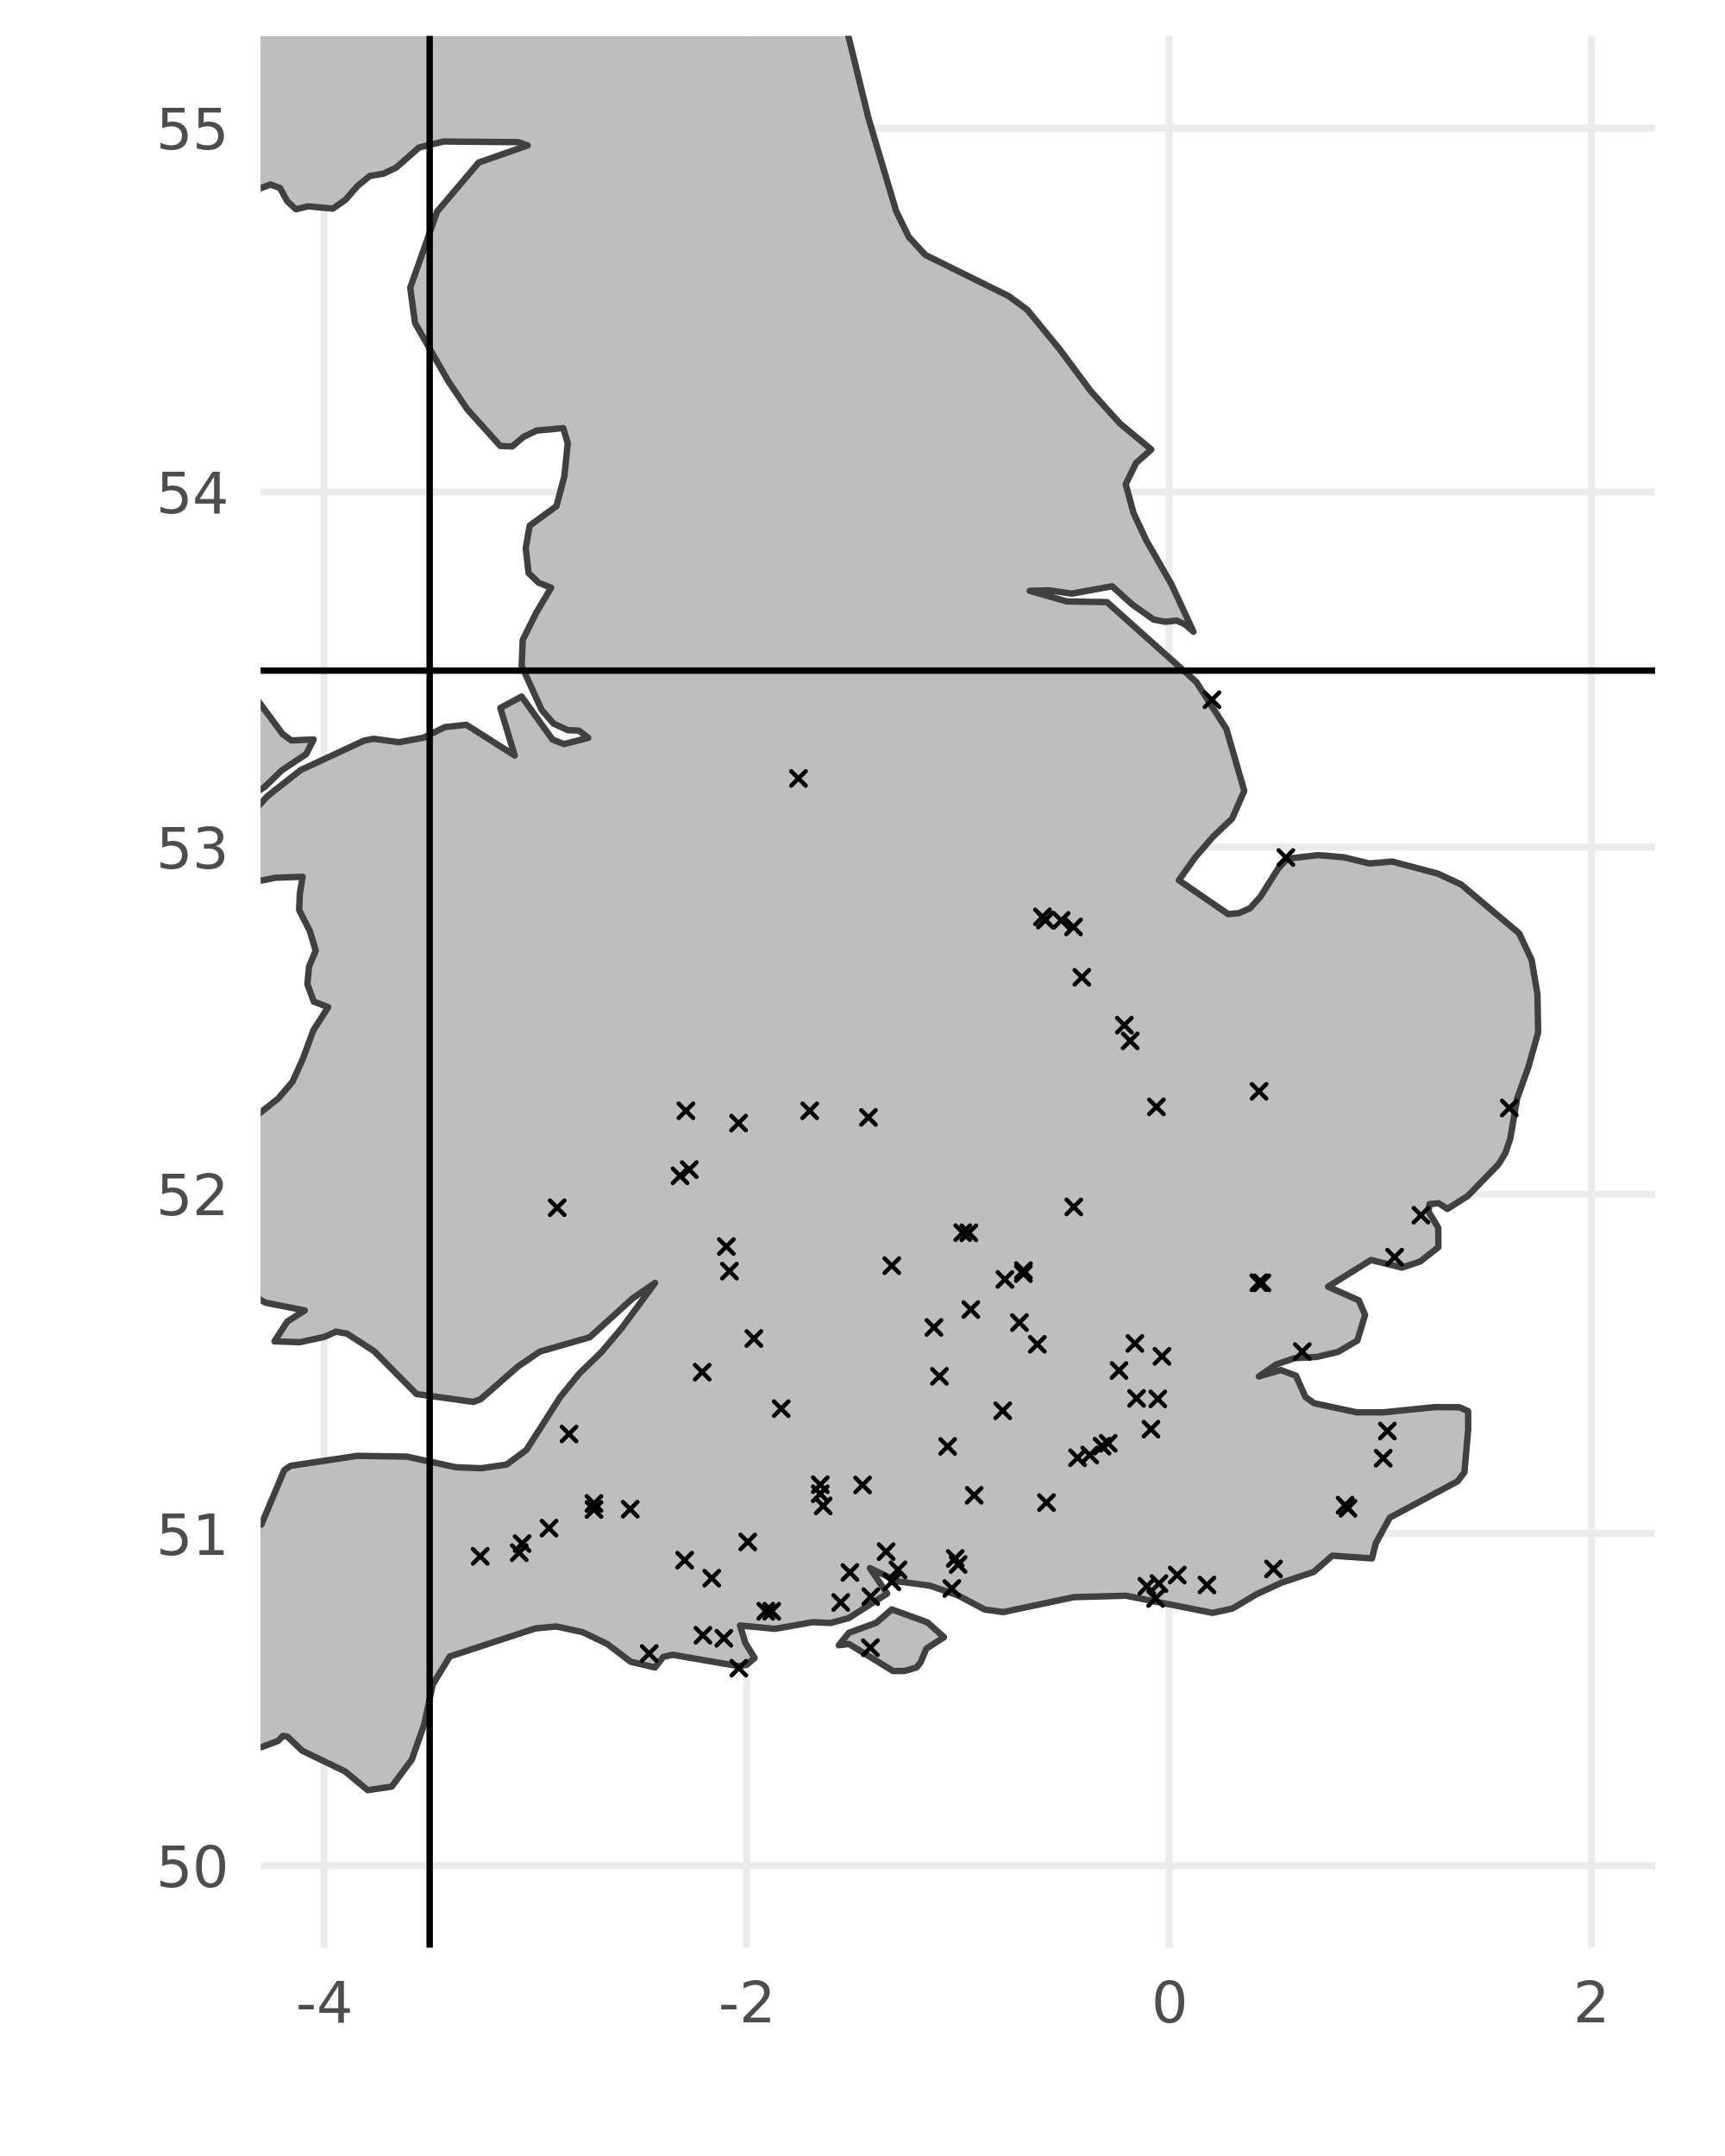
\includegraphics{ButterflyMarkdowns/ButterflySIFigs/ButterflySiteMaps.png}
\caption{Distribution of UKBMS transect sites with sufficient data over
focal period to be included in the analysis.}
\end{figure}

\hypertarget{occupancy-through-time}{%
\subsection{Occupancy Through Time}\label{occupancy-through-time}}

\begin{figure}
\centering
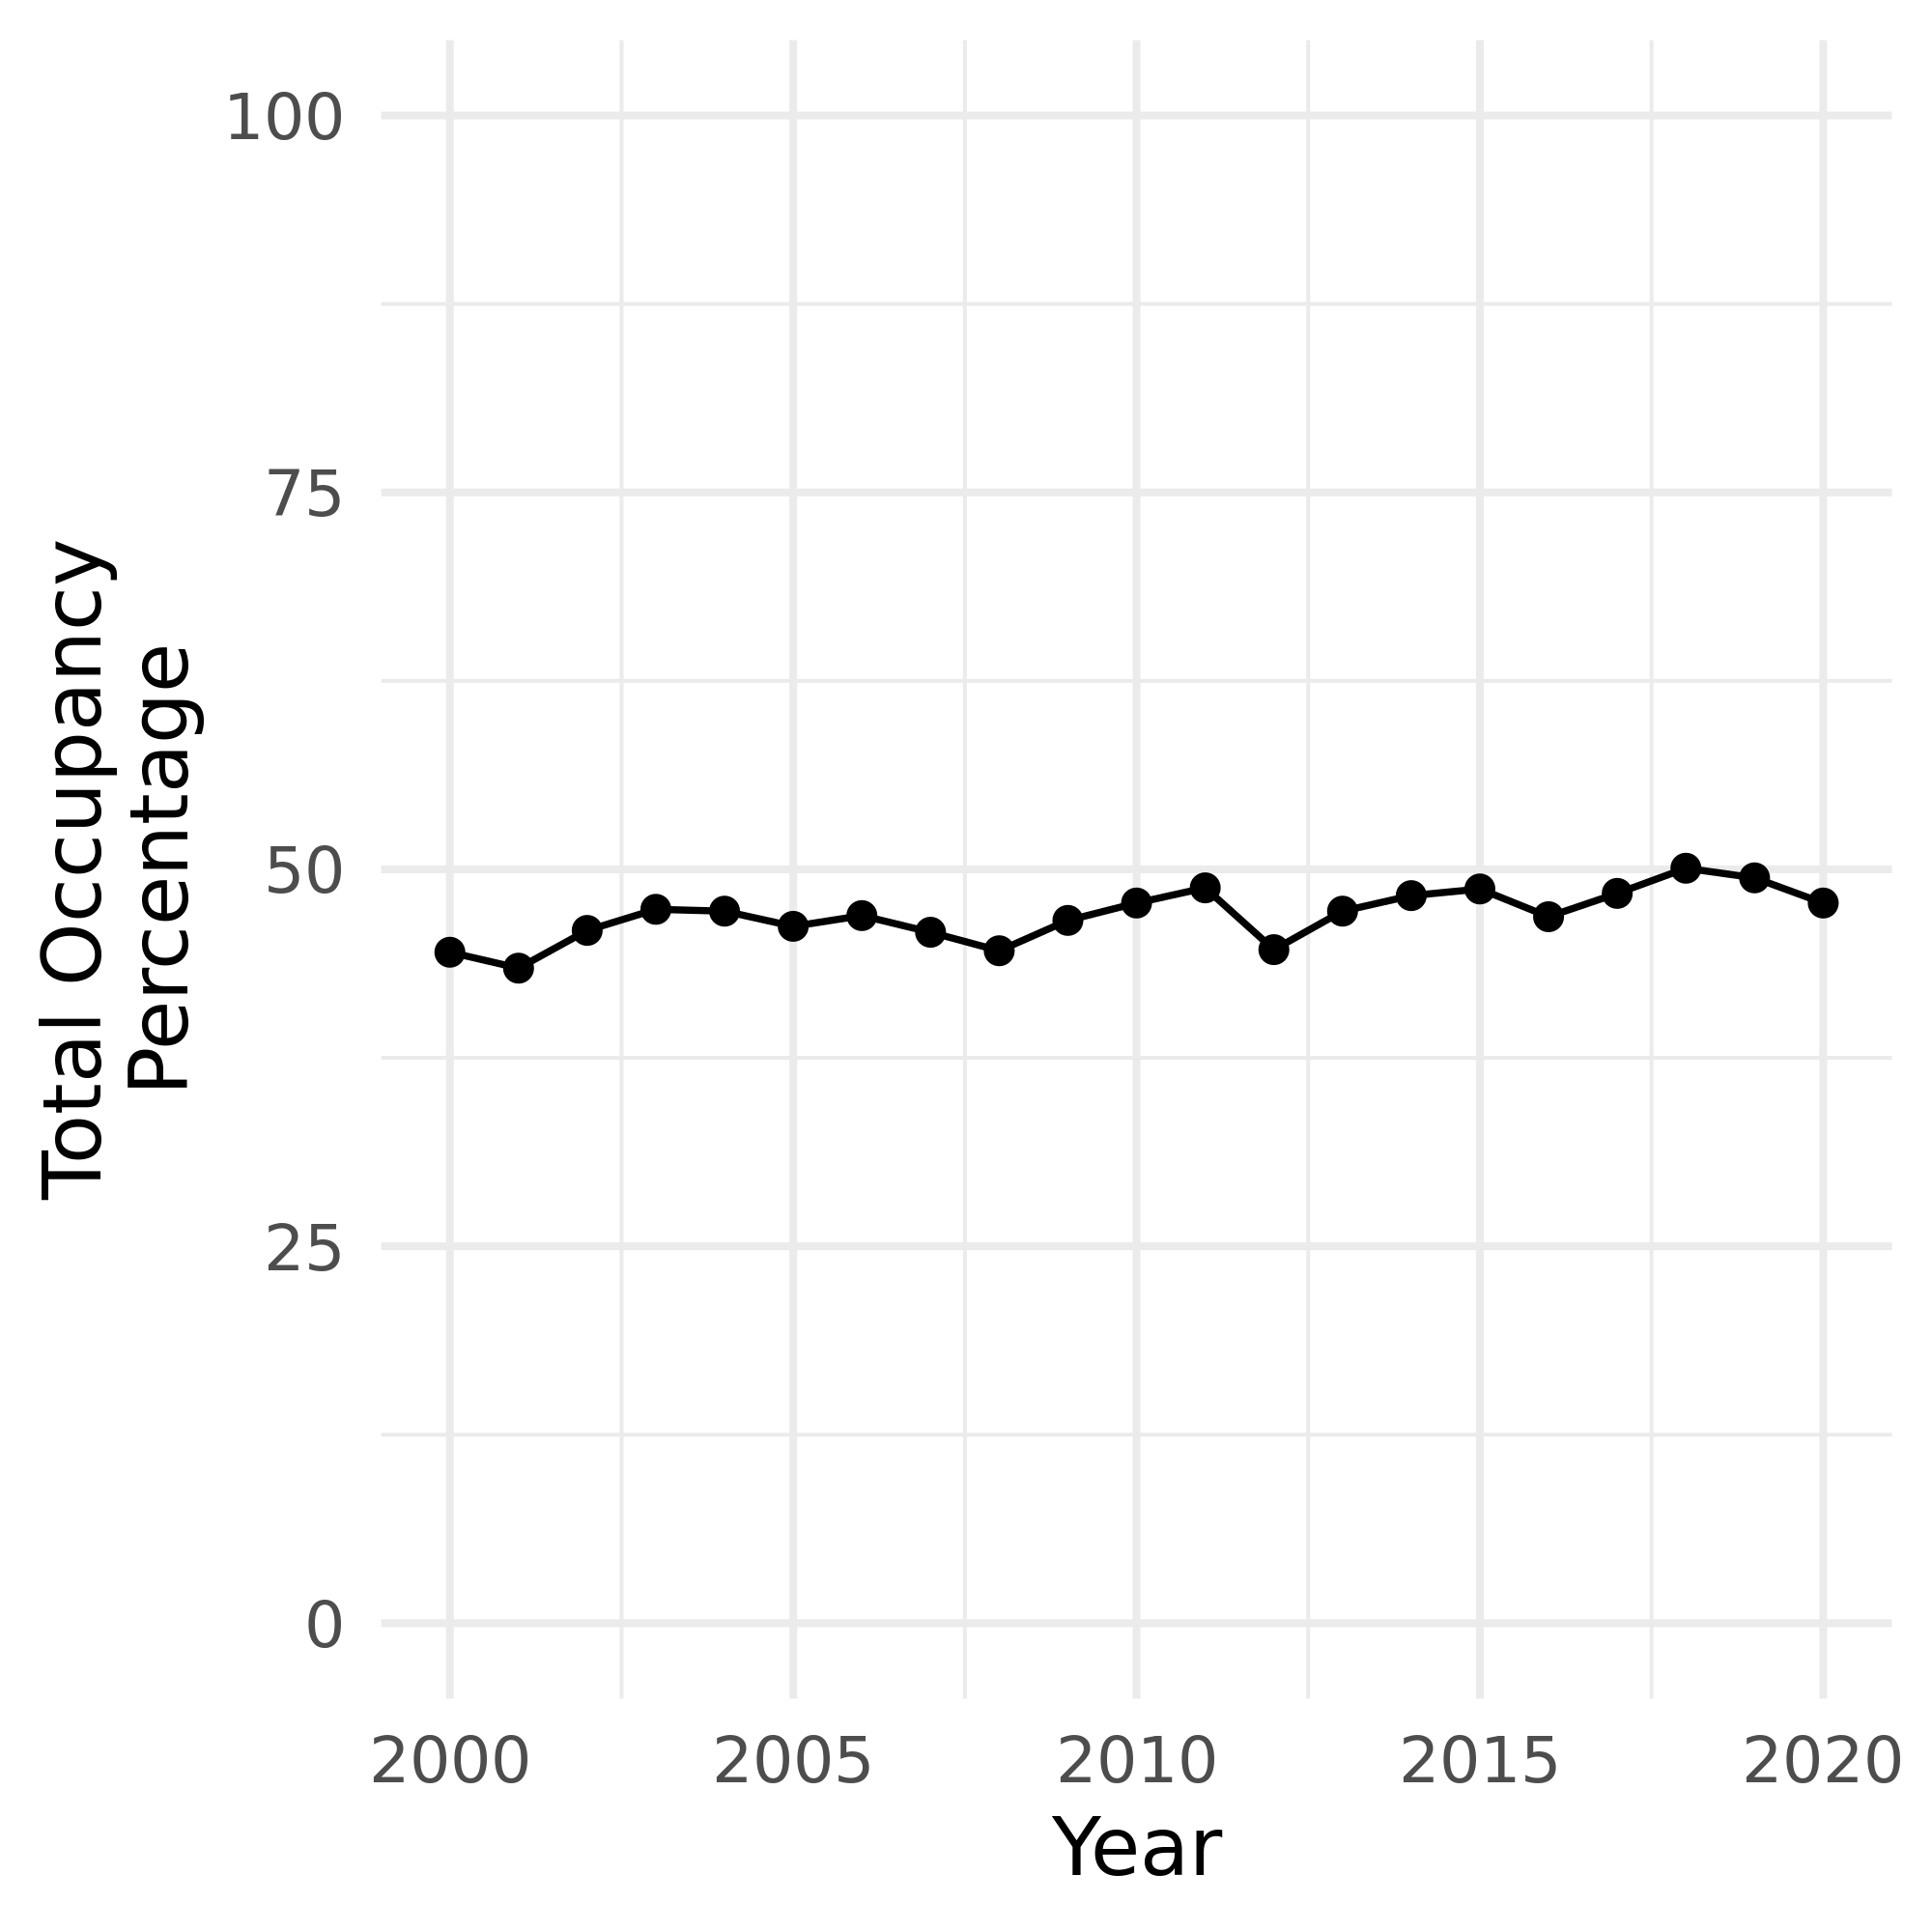
\includegraphics{ButterflyMarkdowns/ButterflySIFigs/TotalOccupancy.png}
\caption{Total occupancy (i.e.~total species:site presence records out
of maximum possible) of focal butterfly species in focal sites across
the time period.}
\end{figure}

\hypertarget{species-level-responses}{%
\subsection{Species-Level Responses}\label{species-level-responses}}

\begin{figure}
\centering
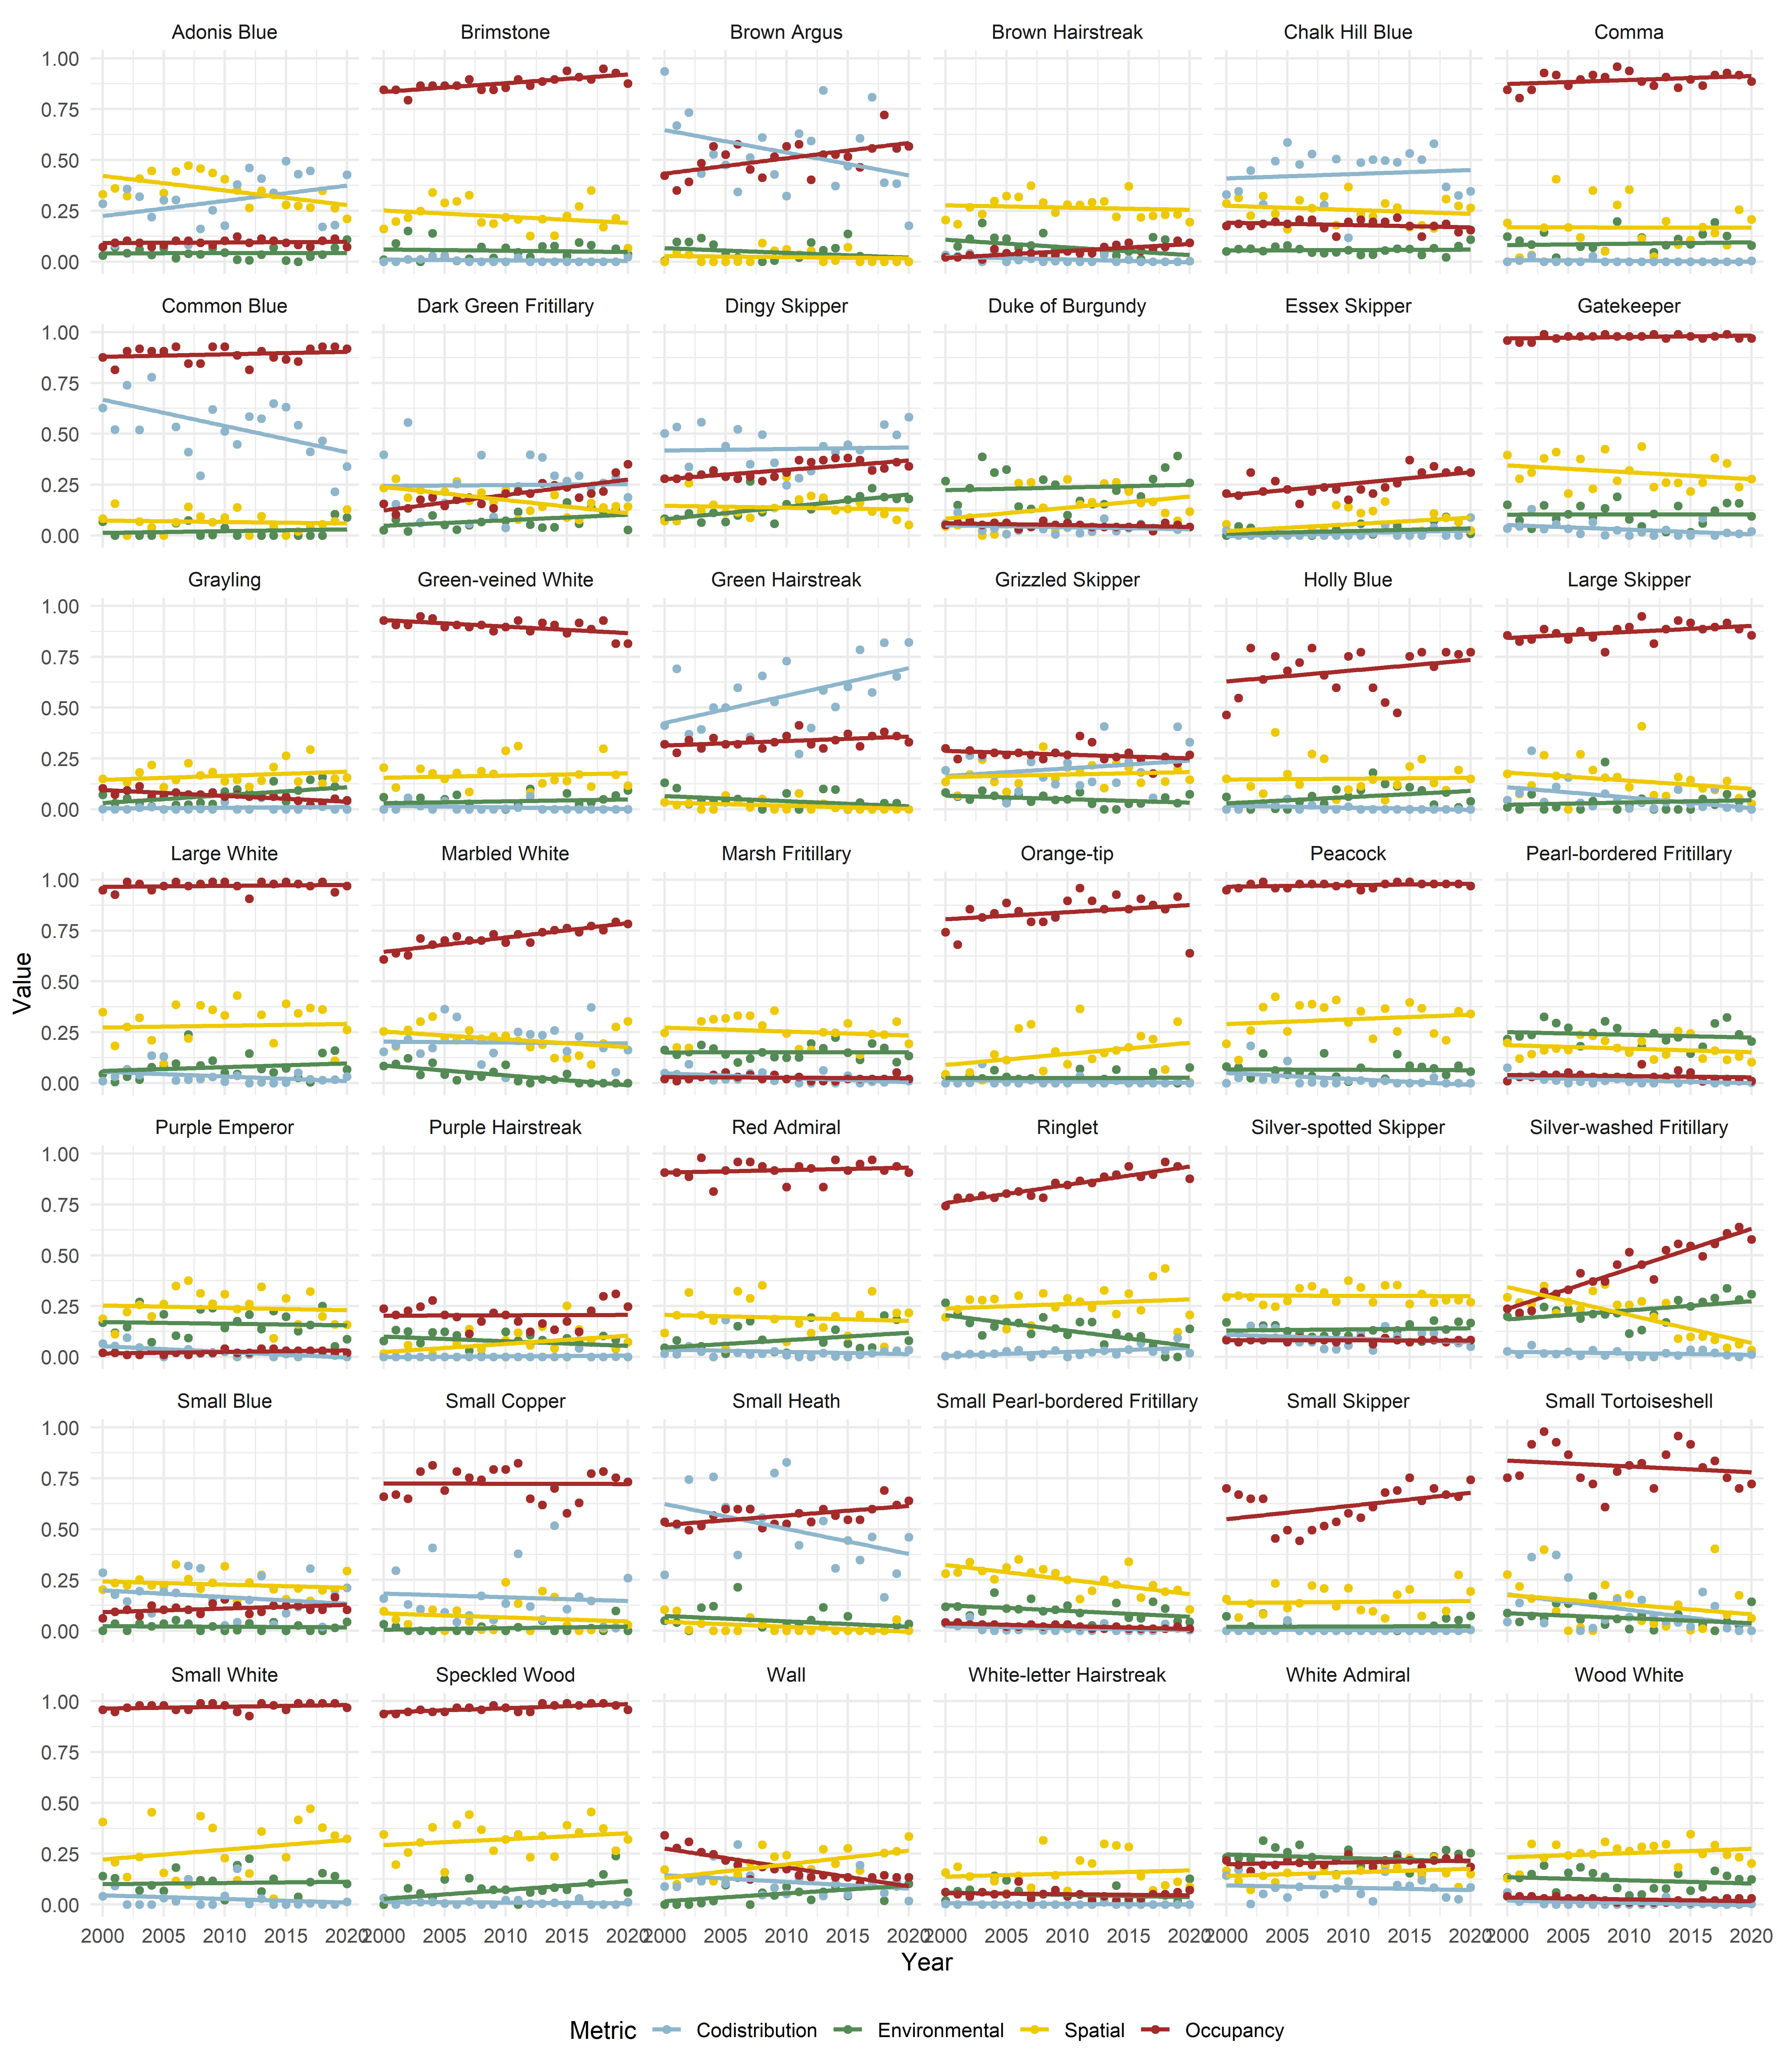
\includegraphics{ButterflyMarkdowns/ButterflySIFigs/SpeciesResponses.png}
\caption{Species-level variance partitioning and species occupancy
fraction (out of the 97 focal sites) through time. Note that the changes
in the overall variance partitioning are driven by changes in relatively
few of the species. However, these species (for example Common Blue and
Green Hairstreak) are not necessarily those that are notably changing
occupancy through this period.}
\end{figure}

\newpage

\hypertarget{species-names}{%
\subsection{Species Names}\label{species-names}}

\begin{longtable}[]{@{}ll@{}}
\caption{Linnean binomials and English common names of focal butterfly
species}\tabularnewline
\toprule
Scientific Name & English Common Name \\
\midrule
\endfirsthead
\toprule
Scientific Name & English Common Name \\
\midrule
\endhead
\textit{Polyommatus bellargus} & Adonis Blue \\
\textit{Gonepteryx rhamni} & Brimstone \\
\textit{Aricia agestis} & Brown Argus \\
\textit{Thecla betulae} & Brown Hairstreak \\
\textit{Polyommatus coridon} & Chalk Hill Blue \\
\textit{Polygonia c-album} & Comma \\
\textit{Polyommatus icarus} & Common Blue \\
\textit{Speyeria aglaja} & Dark Green Fritillary \\
\textit{Erynnis tages} & Dingy Skipper \\
\textit{Hamearis lucina} & Duke of Burgundy \\
\textit{Thymelicus lineola} & Essex Skipper \\
\textit{Pyronia tithonus} & Gatekeeper \\
\textit{Hipparchia semele} & Grayling \\
\textit{Pieris napi} & Green-veined White \\
\textit{Callophrys rubi} & Green Hairstreak \\
\textit{Pyrgus malvae} & Grizzled Skipper \\
\textit{Celastrina argiolus} & Holly Blue \\
\textit{Ochlodes sylvanus} & Large Skipper \\
\textit{Pieris brassicae} & Large White \\
\textit{Melanargia galathea} & Marbled White \\
\textit{Euphydryas aurinia} & Marsh Fritillary \\
\textit{Anthocharis cardamines} & Orange-tip \\
\textit{Aglais io} & Peacock \\
\textit{Boloria euphrosyne} & Pearl-bordered Fritillary \\
\textit{Apatura iris} & Purple Emperor \\
\textit{Favonius quercus} & Purple Hairstreak \\
\textit{Vanessa atalanta} & Red Admiral \\
\textit{Aphantopus hyperantus} & Ringlet \\
\textit{Hesperia comma} & Silver-spotted Skipper \\
\textit{Argynnis paphia} & Silver-washed Fritillary \\
\textit{Cupido minimus} & Small Blue \\
\textit{Lycaena phlaeas} & Small Copper \\
\textit{Coenonympha pamphilus} & Small Heath \\
\textit{Boloria selene} & Small Pearl-bordered Fritillary \\
\textit{Thymelicus sylvestris} & Small Skipper \\
\textit{Aglais urticae} & Small Tortoiseshell \\
\textit{Pieris rapae} & Small White \\
\textit{Pararge aegeria} & Speckled Wood \\
\textit{Lasiommata megera} & Wall \\
\textit{Satyrium w-album} & White-letter Hairstreak \\
\textit{Limenitis camilla} & White Admiral \\
\textit{Leptidea sinapis} & Wood White \\
\bottomrule
\end{longtable}

\hypertarget{fitted-environmental-coefficients}{%
\subsection{Fitted Environmental
Coefficients}\label{fitted-environmental-coefficients}}

\begin{figure}
\centering
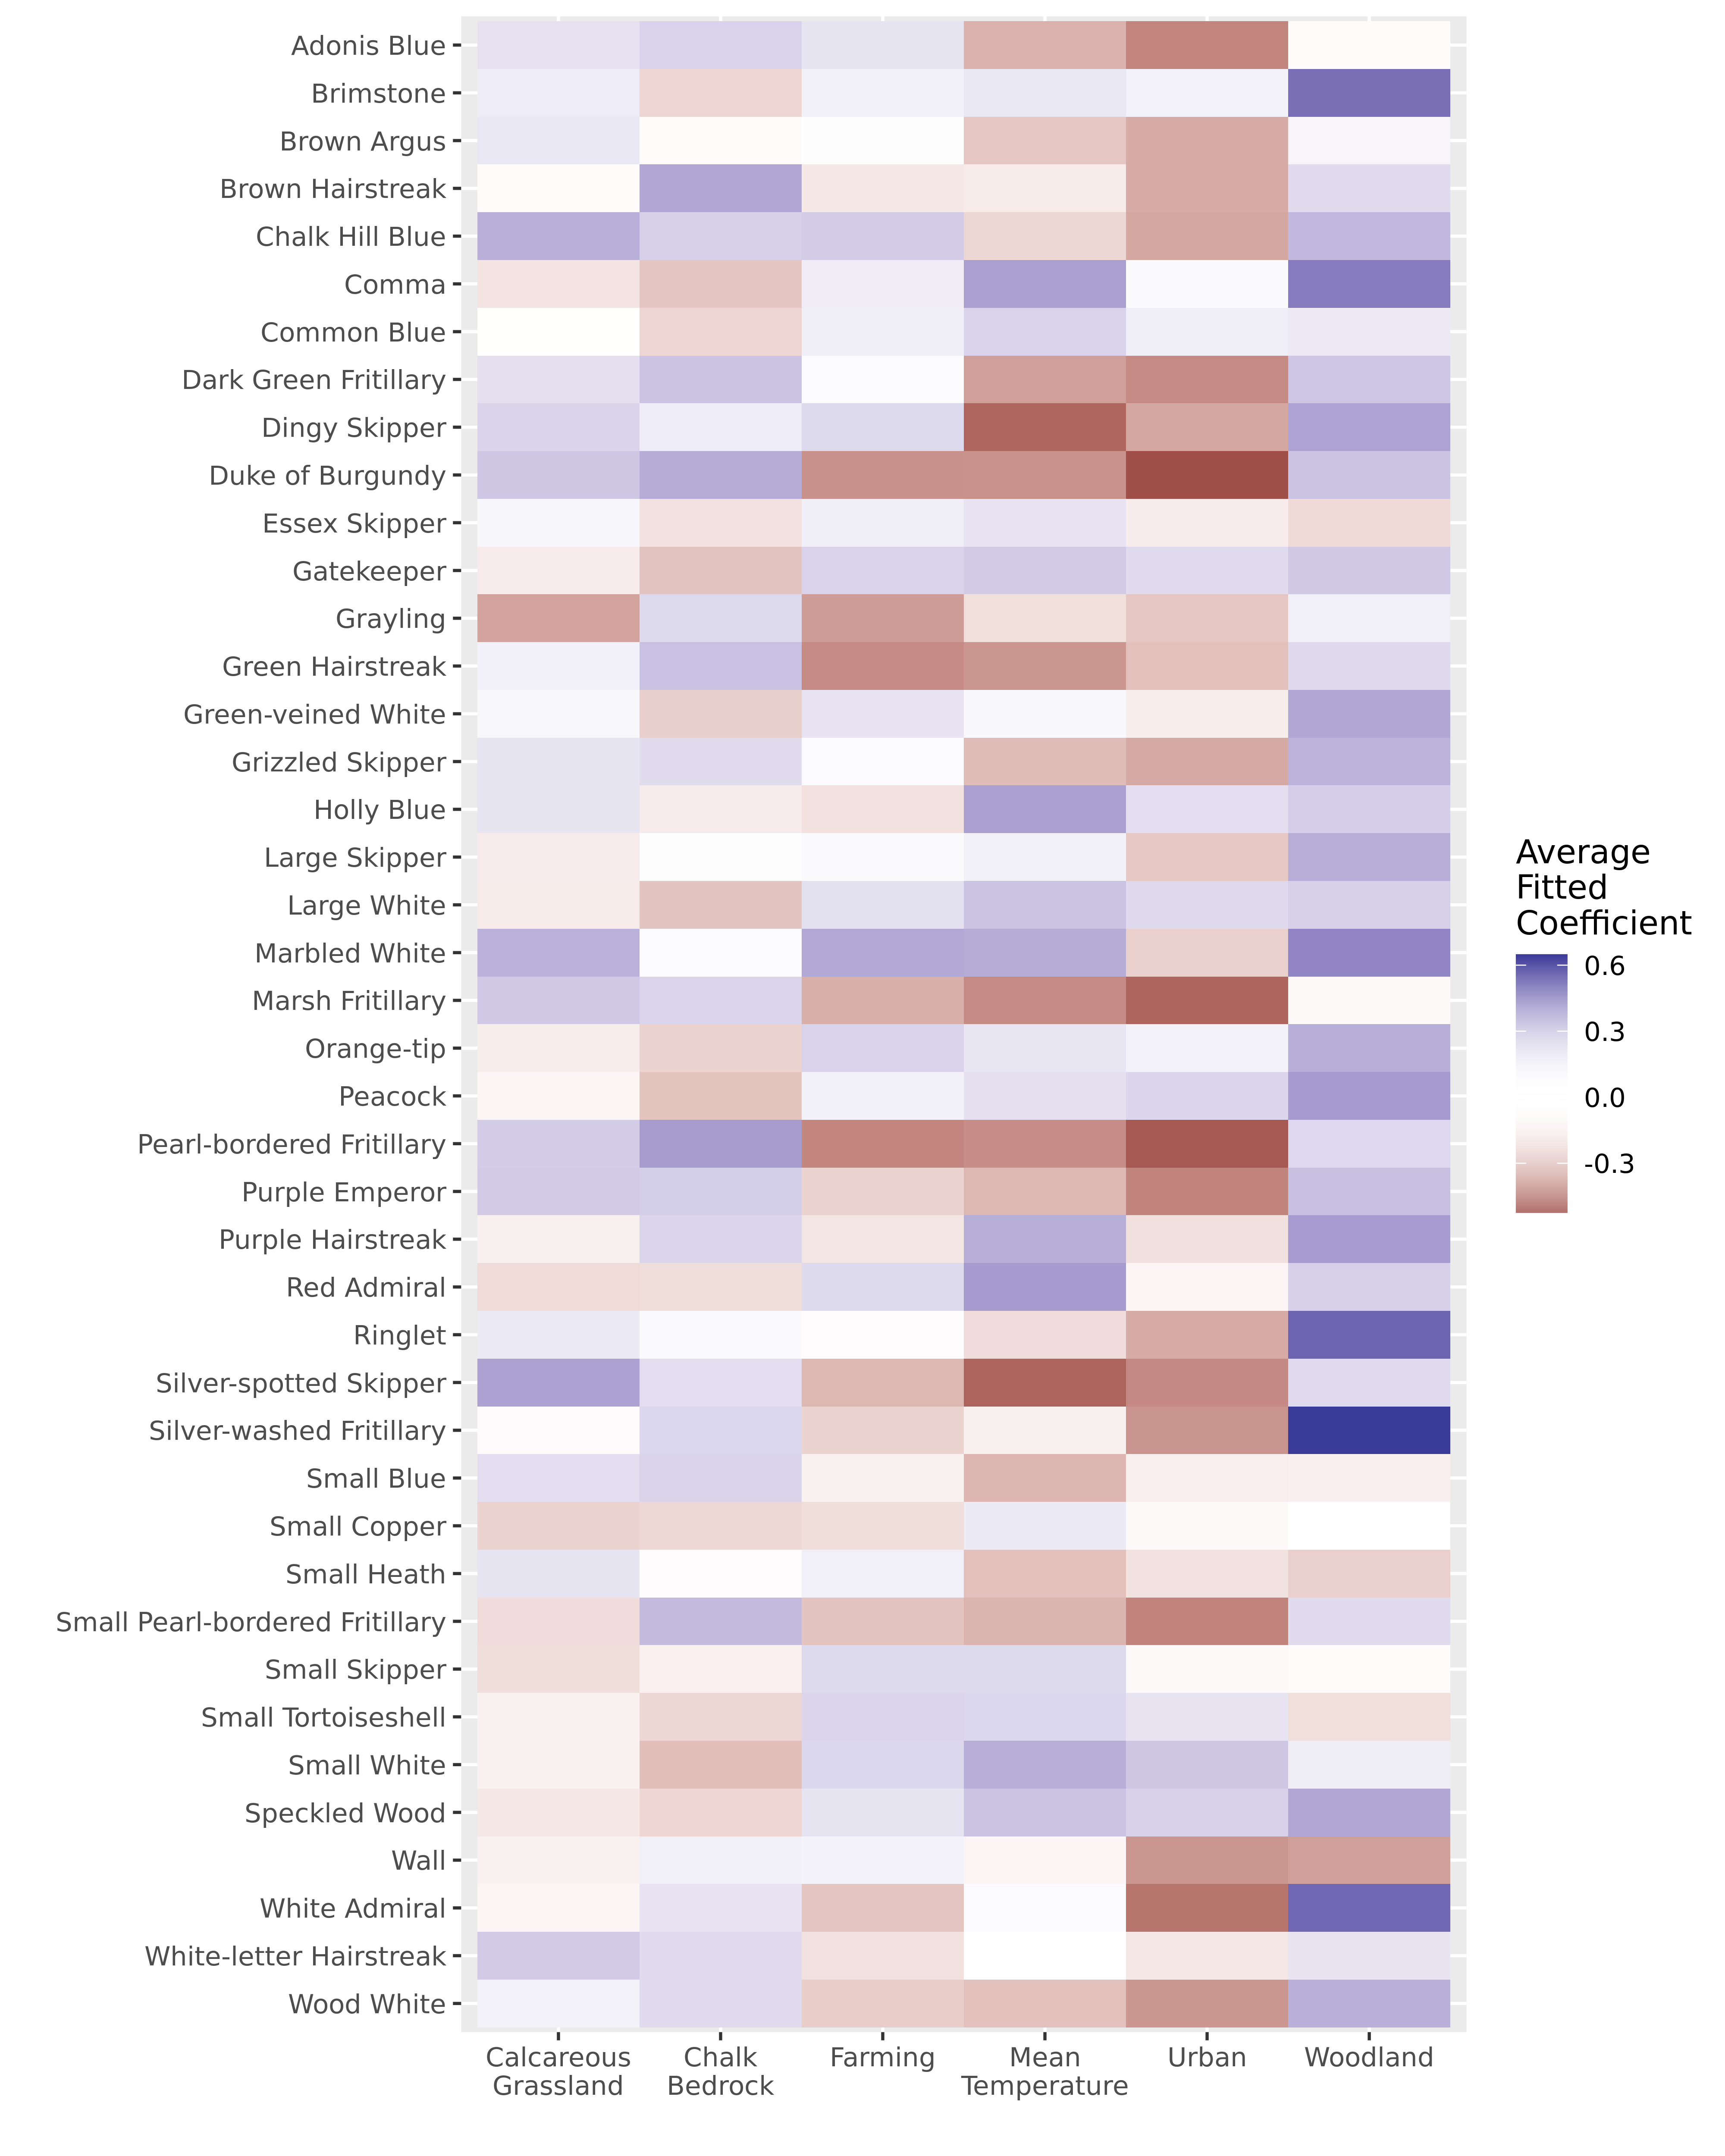
\includegraphics[width=\textwidth,height=0.7\textheight]{ButterflyMarkdowns/ButterflySIFigs/EnvCoeffs.png}
\caption{Butterfly fitted species-level environmental coefficients,
averaged across all 21 years.}
\end{figure}

\hypertarget{fitted-species-associations}{%
\subsection{Fitted Species
Associations}\label{fitted-species-associations}}

\begin{figure}
\centering
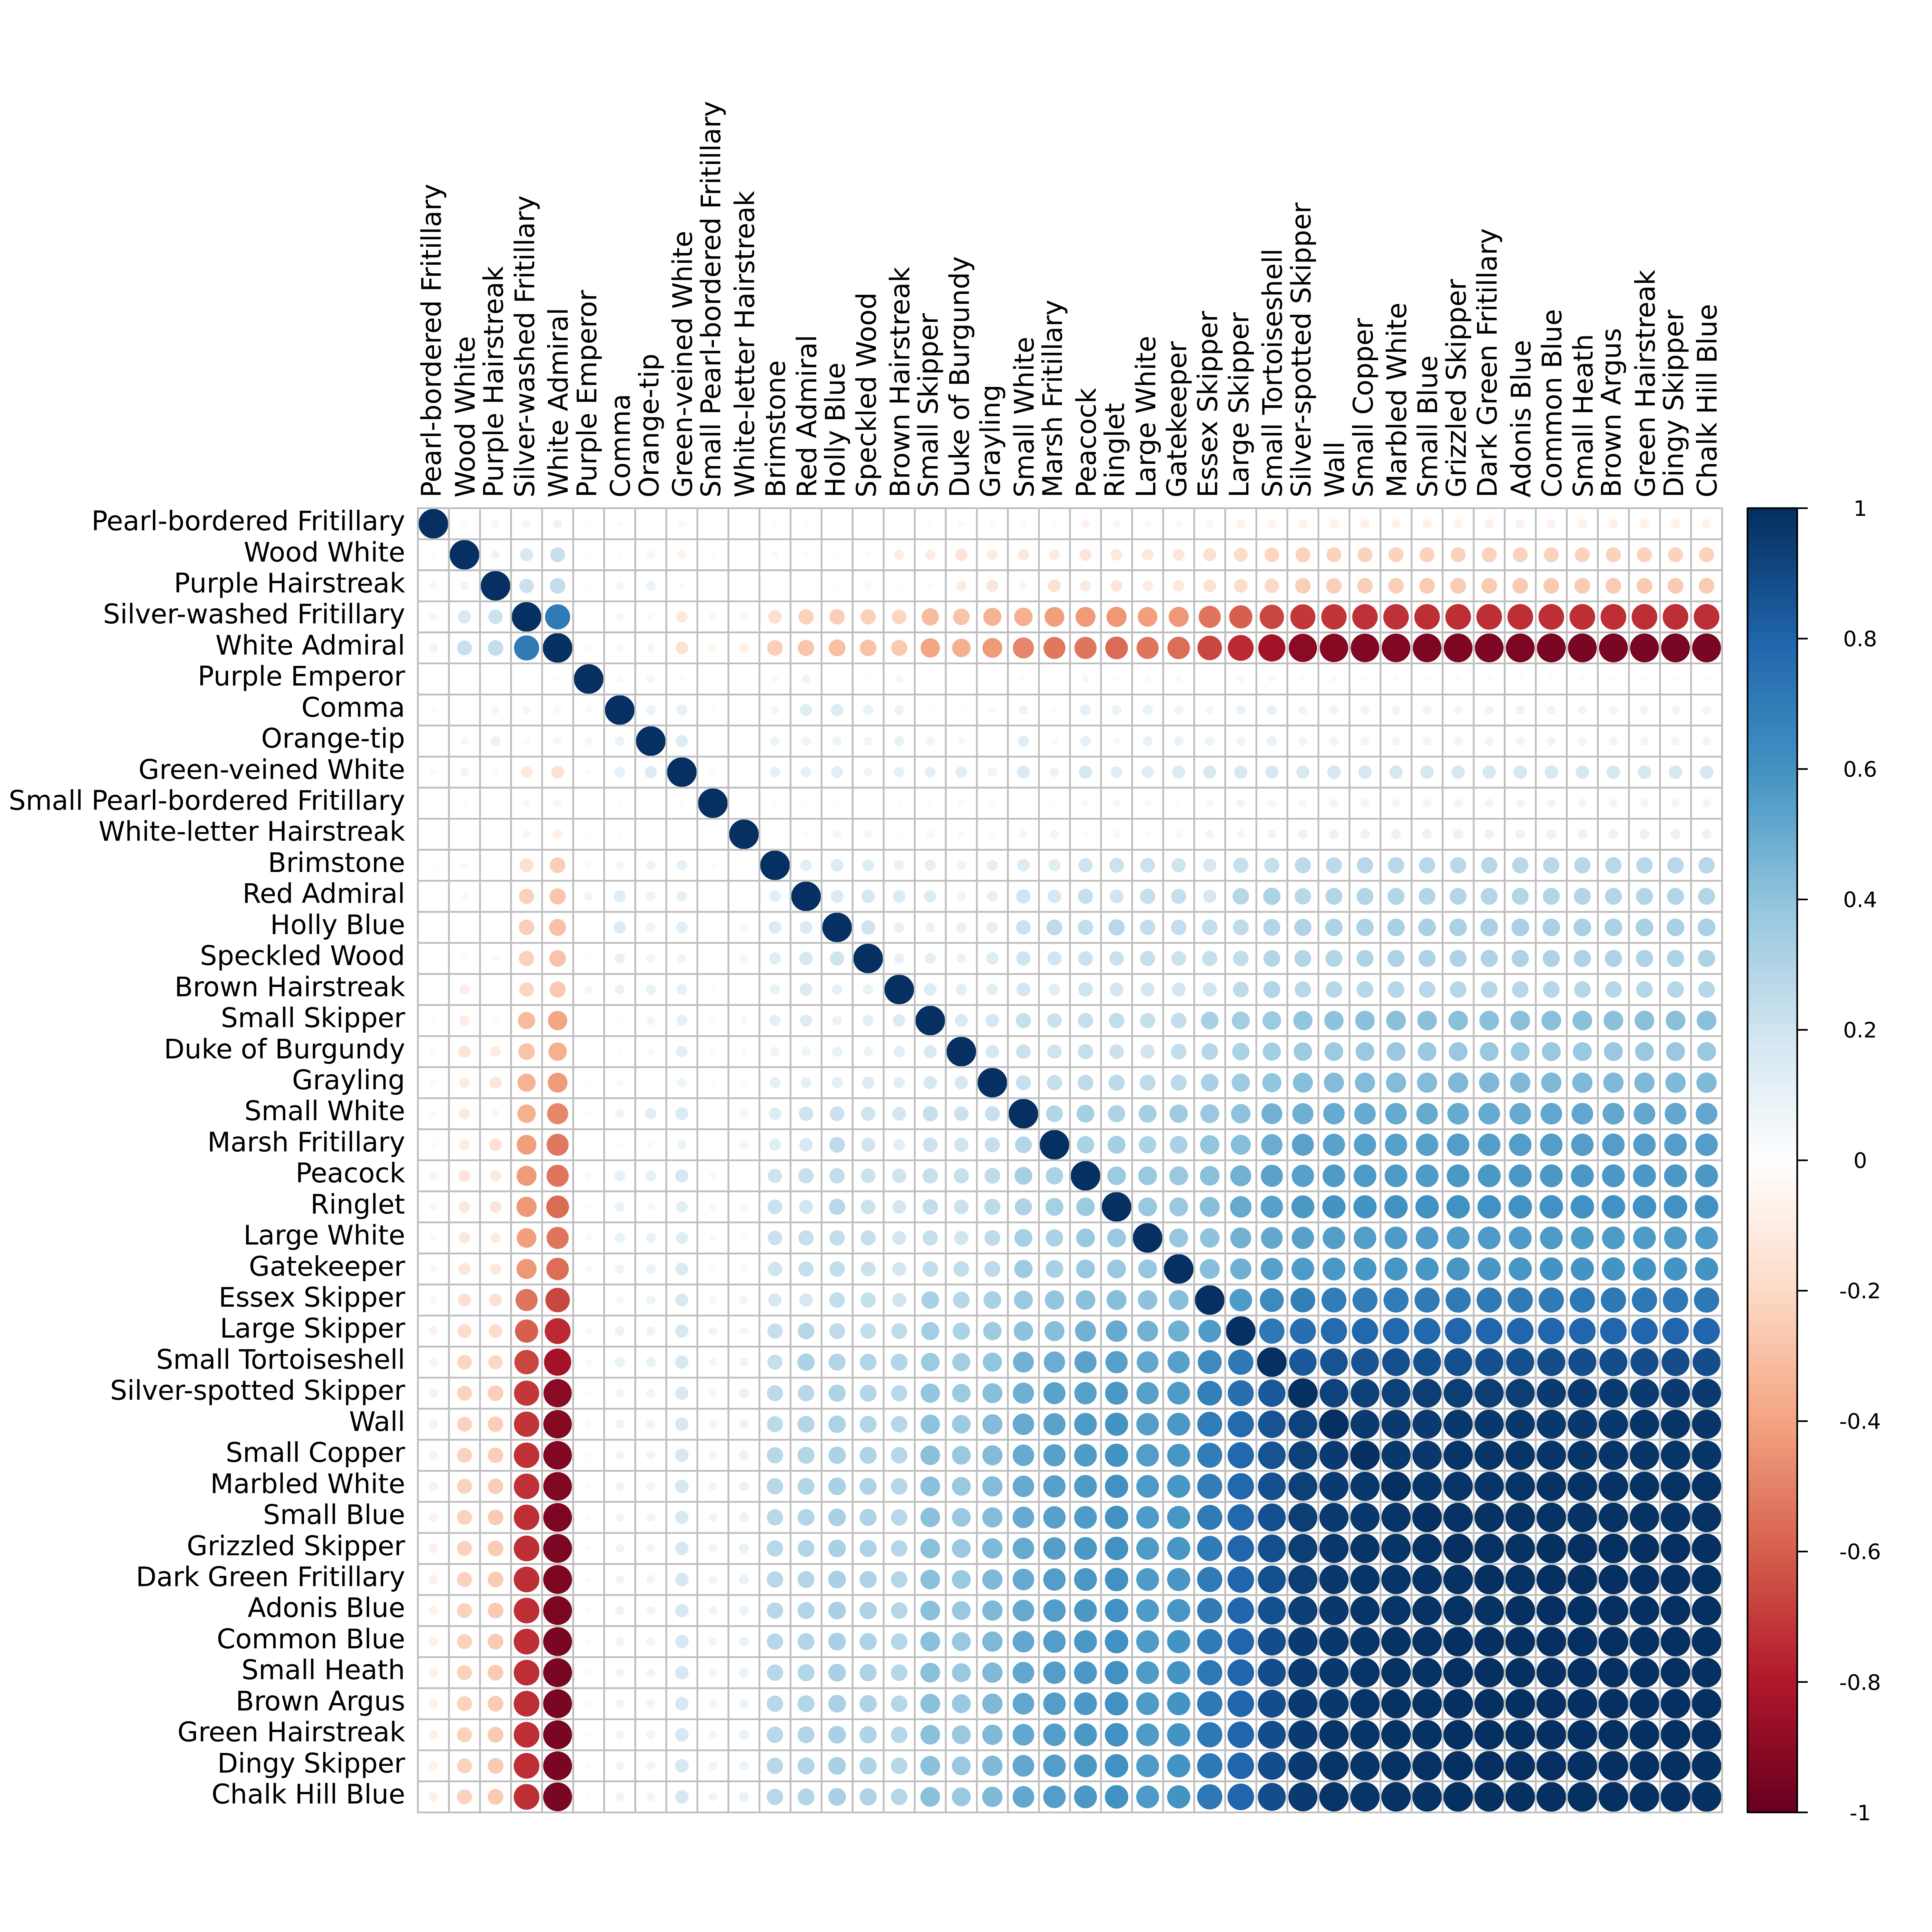
\includegraphics[width=\textwidth,height=0.8\textheight]{ButterflyMarkdowns/ButterflySIFigs/SpAssCoeffs.png}
\caption{Fitted residual species associations defined by a correlation
matrix, averaged across all time slices. Note the grouping into a large
cluster dominated by chalk grassland species (bottom right) and a
smaller cluster of species (top left) associated with woodlands.}
\end{figure}

\hypertarget{confirming-model-convergence}{%
\subsection{Confirming Model
Convergence}\label{confirming-model-convergence}}

\begin{figure}
\centering
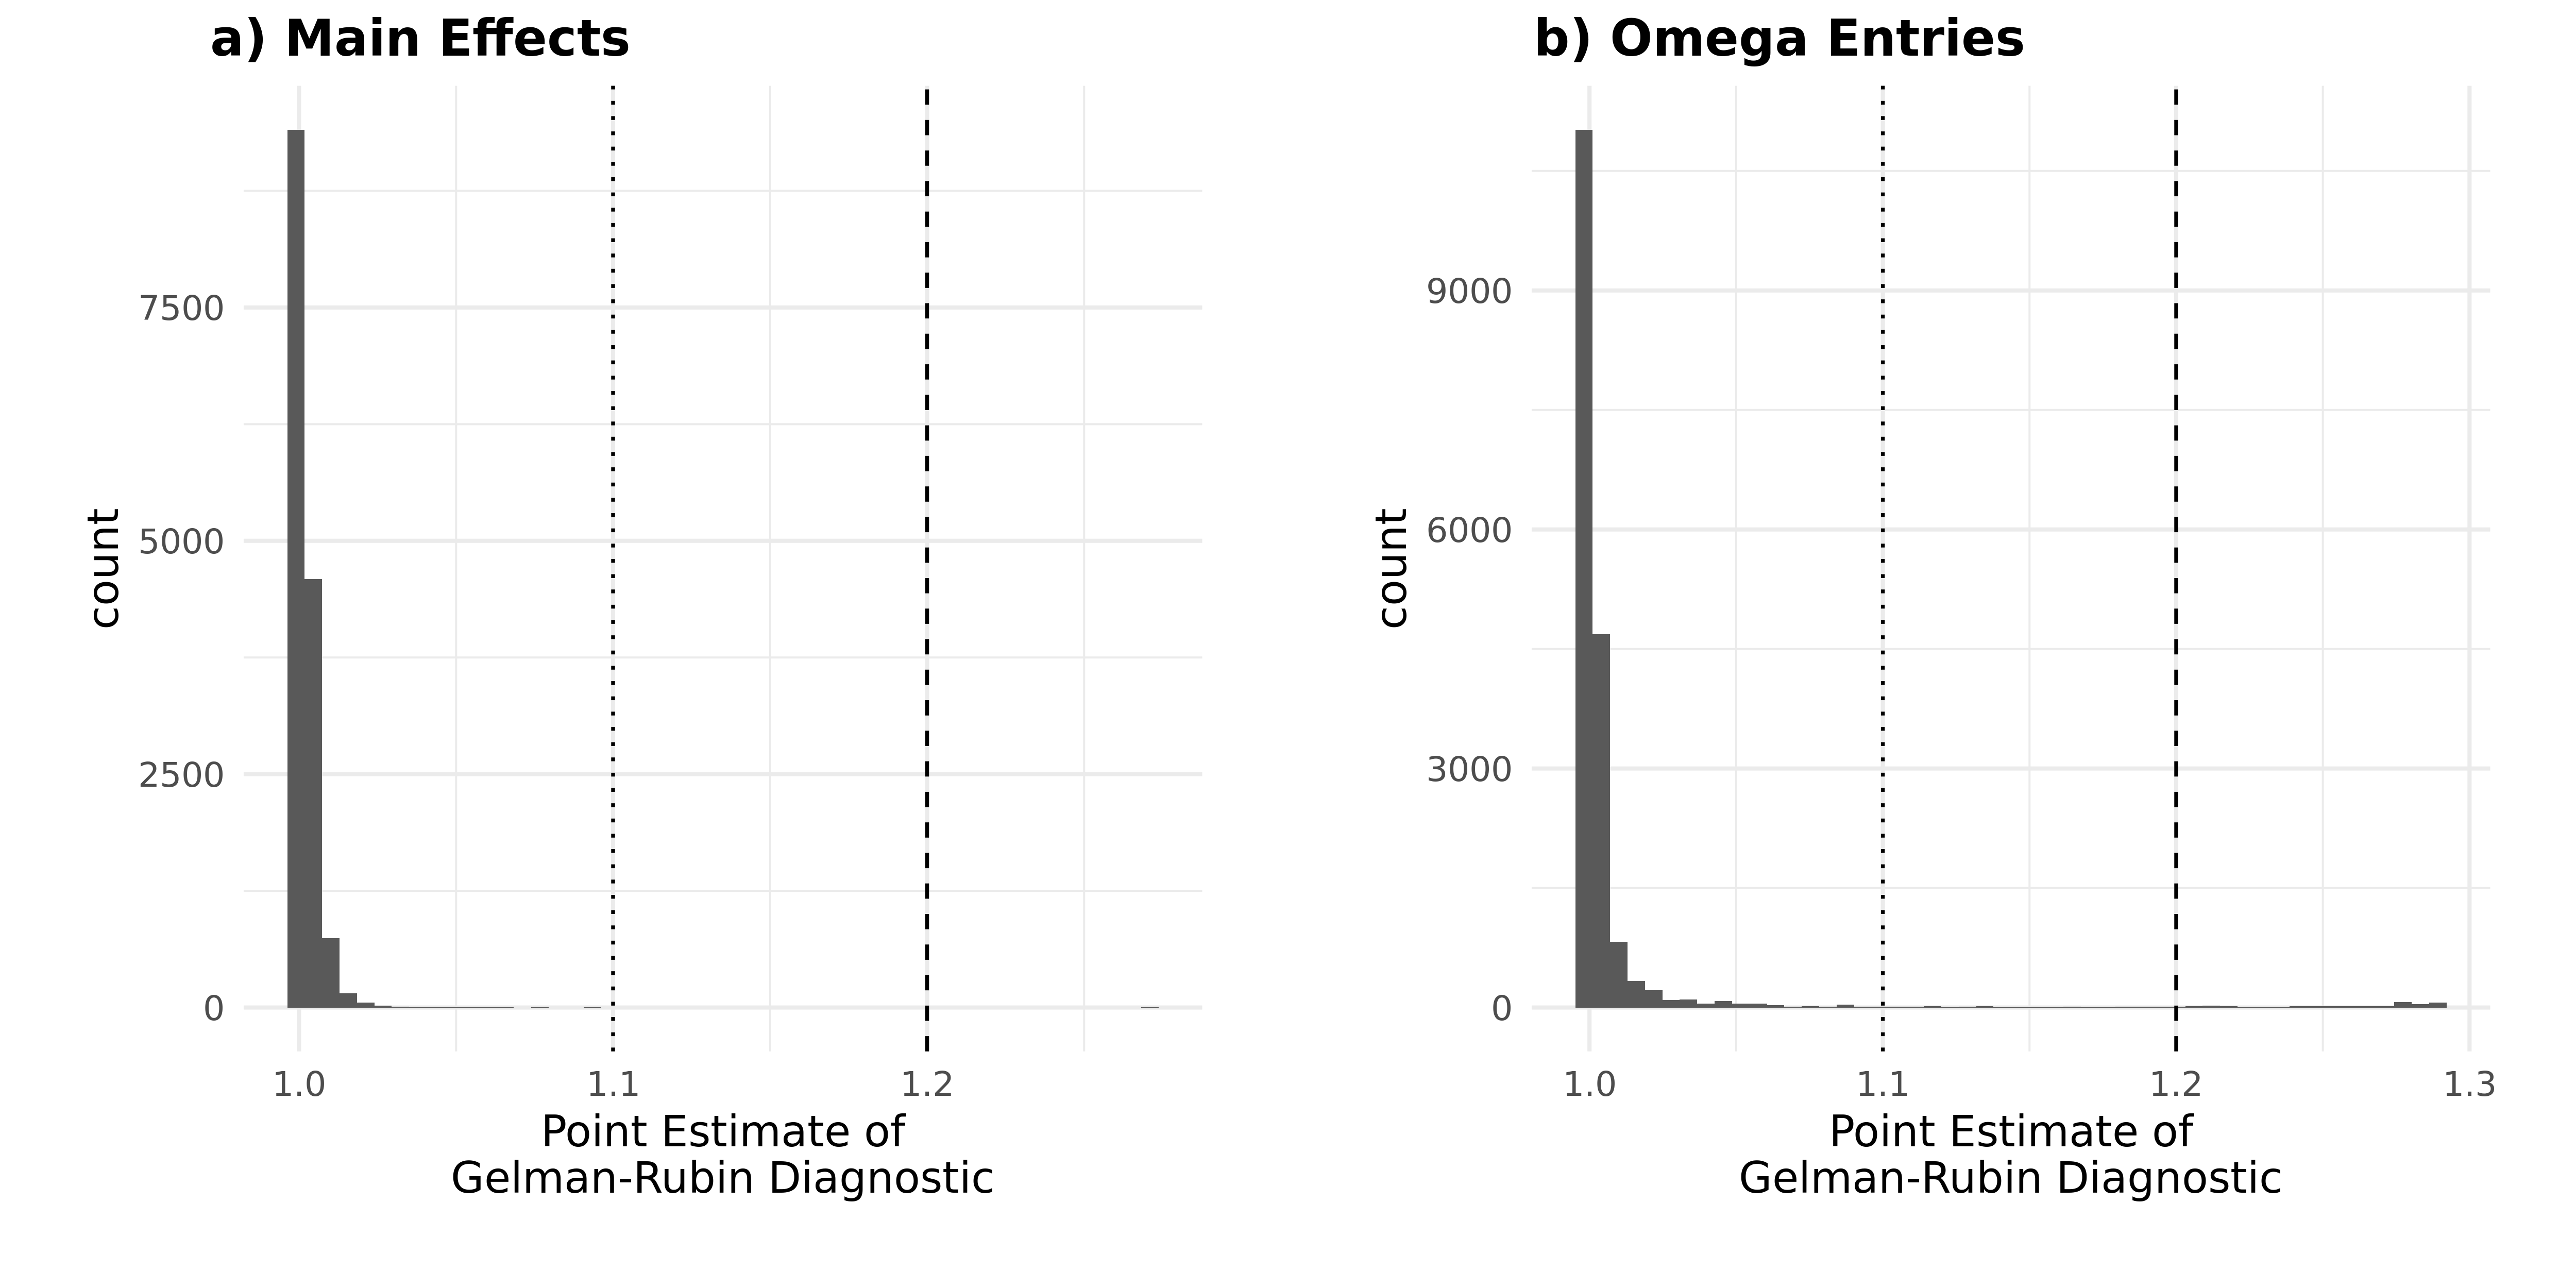
\includegraphics{ButterflyMarkdowns/ButterflySIFigs/ButterflyConvergence_GR.png}
\caption{Histogram of Gelman-Rubin MCMC convergence statistics across
all years of the butterfly dataset based on two independent chains fit
for each year of the full model (total iterations = 100000, burn-in =
50000, and thinning = 50) a) Main effect coefficients
(i.e.~environmental and spatial coefficients) are all well below the
standard threshold of 1.1, indicating acceptable convergence. b)
Equivalent results for the species codistribution fitting are by
necessity slightly more derived, as they are fit by latent variables
that might not necessarily be fit in the same order, even if they
converge. We therefore examine the convergence in the elements of the
correlation matrix \(\Omega\). Here the vast majority are well
converged, although there are a few correlations that exceeded 1.2.
However, as these were very much a minority and were not signifcantly
over (the maximum was 1.29), we considered these models suitable
converged.}
\end{figure}

\hypertarget{bird-dataset}{%
\section{Bird Dataset}\label{bird-dataset}}

\hypertarget{distribution-of-sites-1}{%
\subsection{Distribution of Sites}\label{distribution-of-sites-1}}

\begin{figure}
\centering
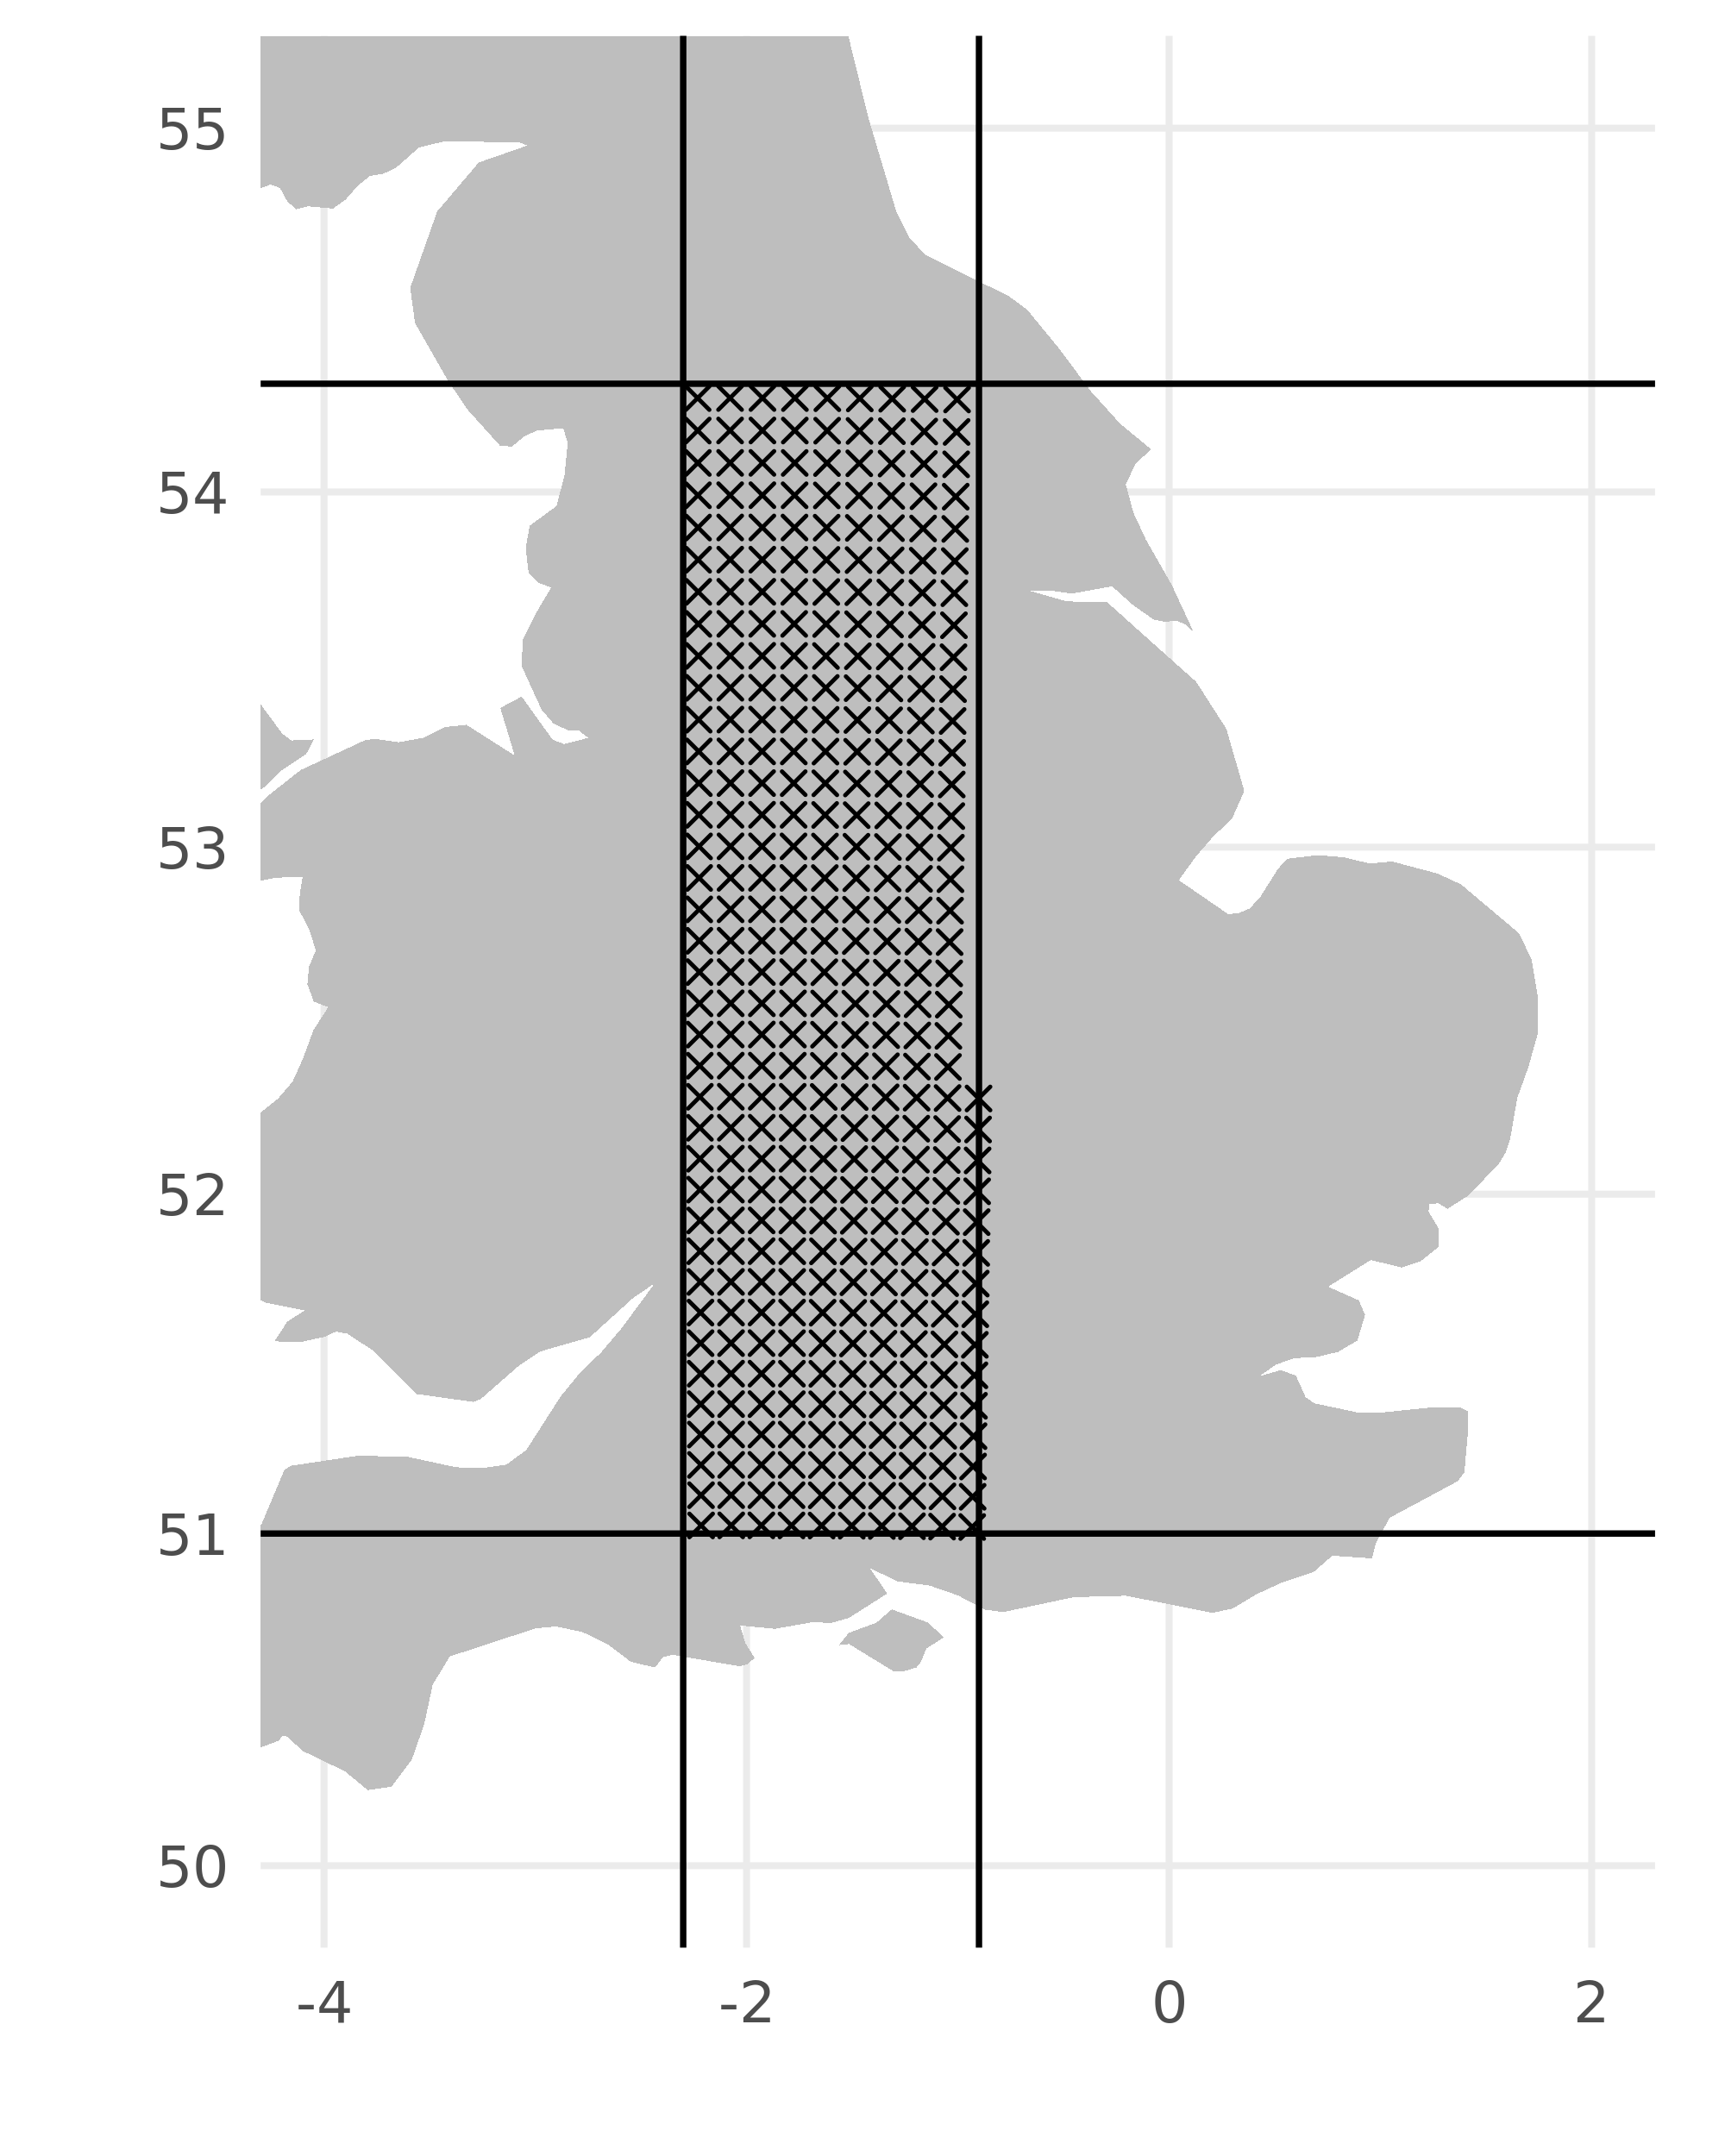
\includegraphics{BirdMarkdowns/BirdImages/HectadLocations.png}
\caption{Location of the hectads retained from the British Breeding Bird
Atlas dataset. Boundaries (51° : 54.3° latitude, -2.3° : -0.9°
longitude) were chosen to be a simple shape that excludes coastal
regions. The slight shoulder is due to the non-exact alignment between
the UK National Grid and lines of longitude.}
\end{figure}

\newpage

\hypertarget{species-names-1}{%
\subsection{Species Names}\label{species-names-1}}

\begin{longtable}[]{@{}lll@{}}
\caption{Linnean binomials and English common names of focal bird
species. ``HQ'' column indicates if the species had sufficient
``high-quality'' observations to be retained in the more restricted
datasets.}\tabularnewline
\toprule
Scientific Name & English Common Name & HQ \\
\midrule
\endfirsthead
\toprule
Scientific Name & English Common Name & HQ \\
\midrule
\endhead
\textit{Tyto alba} & Barn Owl & TRUE \\
\textit{Chroicocephalus ridibundus} & Black-headed Gull & TRUE \\
\textit{Lyrurus tetrix} & Black Grouse & FALSE \\
\textit{Phoenicurus ochruros} & Black Redstart & TRUE \\
\textit{Branta canadensis} & Canada Goose & TRUE \\
\textit{Actitis hypoleucos} & Common Sandpiper & TRUE \\
\textit{Sterna hirundo} & Common Tern & TRUE \\
\textit{Fulica atra} & Coot & TRUE \\
\textit{Emberiza calandra} & Corn Bunting & TRUE \\
\textit{Numenius arquata} & Curlew & TRUE \\
\textit{Cinclus cinclus} & Dipper & TRUE \\
\textit{Calidris alpina} & Dunlin & TRUE \\
\textit{Mareca strepera} & Gadwall & FALSE \\
\textit{Spatula querquedula} & Garganey & TRUE \\
\textit{Regulus regulus} & Goldcrest & TRUE \\
\textit{Pluvialis apricaria} & Golden Plover & TRUE \\
\textit{Accipiter gentilis} & Goshawk & TRUE \\
\textit{Locustella naevia} & Grasshopper Warbler & TRUE \\
\textit{Podiceps cristatus} & Great Crested Grebe & TRUE \\
\textit{Picus viridis} & Green Woodpecker & TRUE \\
\textit{Ardea cinerea} & Grey Heron & TRUE \\
\textit{Perdix perdix} & Grey Partridge & TRUE \\
\textit{Motacilla cinerea} & Grey Wagtail & TRUE \\
\textit{Anser anser} & Greylag Goose & TRUE \\
\textit{Coccothraustes coccothraustes} & Hawfinch & TRUE \\
\textit{Circus cyaneus} & Hen Harrier & FALSE \\
\textit{Falco subbuteo} & Hobby & TRUE \\
\textit{Garrulus glandarius} & Jay & TRUE \\
\textit{Alcedo atthis} & Kingfisher & TRUE \\
\textit{Larus fuscus} & Lesser Black-backed Gull & FALSE \\
\textit{Acanthis cabaret} & Lesser Redpoll & TRUE \\
\textit{Dryobates minor} & Lesser Spotted Woodpecker & TRUE \\
\textit{Sylvia curruca} & Lesser Whitethroat & TRUE \\
\textit{Tachybaptus ruficollis} & Little Grebe & TRUE \\
\textit{Charadrius dubius} & Little Ringed Plover & TRUE \\
\textit{Asio otus} & Long-eared Owl & TRUE \\
\textit{Poecile palustris} & Marsh Tit & TRUE \\
\textit{Anthus pratensis} & Meadow Pipit & TRUE \\
\textit{Falco columbarius} & Merlin & TRUE \\
\textit{Cygnus olor} & Mute Swan & TRUE \\
\textit{Luscinia megarhynchos} & Nightingale & TRUE \\
\textit{Caprimulgus europaeus} & Nightjar & TRUE \\
\textit{Sitta europaea} & Nuthatch & TRUE \\
\textit{Haematopus ostralegus} & Oystercatcher & TRUE \\
\textit{Ficedula hypoleuca} & Pied Flycatcher & TRUE \\
\textit{Aythya ferina} & Pochard & TRUE \\
\textit{Coturnix coturnix} & Quail & TRUE \\
\textit{Corvus corax} & Raven & FALSE \\
\textit{Lagopus lagopus} & Red Grouse & TRUE \\
\textit{Tringa totanus} & Redshank & TRUE \\
\textit{Phoenicurus phoenicurus} & Redstart & TRUE \\
\textit{Emberiza schoeniclus} & Reed Bunting & TRUE \\
\textit{Acrocephalus scirpaceus} & Reed Warbler & TRUE \\
\textit{Turdus torquatus} & Ring Ouzel & TRUE \\
\textit{Charadrius hiaticula} & Ringed Plover & TRUE \\
\textit{Columba livia} & Rock Dove & TRUE \\
\textit{Riparia riparia} & Sand Martin & TRUE \\
\textit{Acrocephalus schoenobaenus} & Sedge Warbler & TRUE \\
\textit{Tadorna tadorna} & Shelduck & FALSE \\
\textit{Asio flammeus} & Short-eared Owl & TRUE \\
\textit{Spatula clypeata} & Shoveler & TRUE \\
\textit{Spinus spinus} & Siskin & FALSE \\
\textit{Gallinago gallinago} & Snipe & TRUE \\
\textit{Burhinus oedicnemus} & Stone-curlew & TRUE \\
\textit{Saxicola rubicola} & Stonechat & TRUE \\
\textit{Anas crecca} & Teal & TRUE \\
\textit{Anthus trivialis} & Tree Pipit & TRUE \\
\textit{Passer montanus} & Tree Sparrow & TRUE \\
\textit{Aythya fuligula} & Tufted Duck & TRUE \\
\textit{Streptopelia turtur} & Turtle Dove & TRUE \\
\textit{Linaria flavirostris} & Twite & TRUE \\
\textit{Rallus aquaticus} & Water Rail & TRUE \\
\textit{Oenanthe oenanthe} & Wheatear & TRUE \\
\textit{Saxicola rubetra} & Whinchat & TRUE \\
\textit{Mareca penelope} & Wigeon & FALSE \\
\textit{Poecile montanus} & Willow Tit & TRUE \\
\textit{Phylloscopus sibilatrix} & Wood Warbler & TRUE \\
\textit{Scolopax rusticola} & Woodcock & TRUE \\
\textit{Lullula arborea} & Woodlark & TRUE \\
\textit{Motacilla flava} & Yellow Wagtail & TRUE \\
\bottomrule
\end{longtable}

\hypertarget{species-habitat-associations}{%
\subsection{Species Habitat
Associations}\label{species-habitat-associations}}

\begin{figure}
\centering
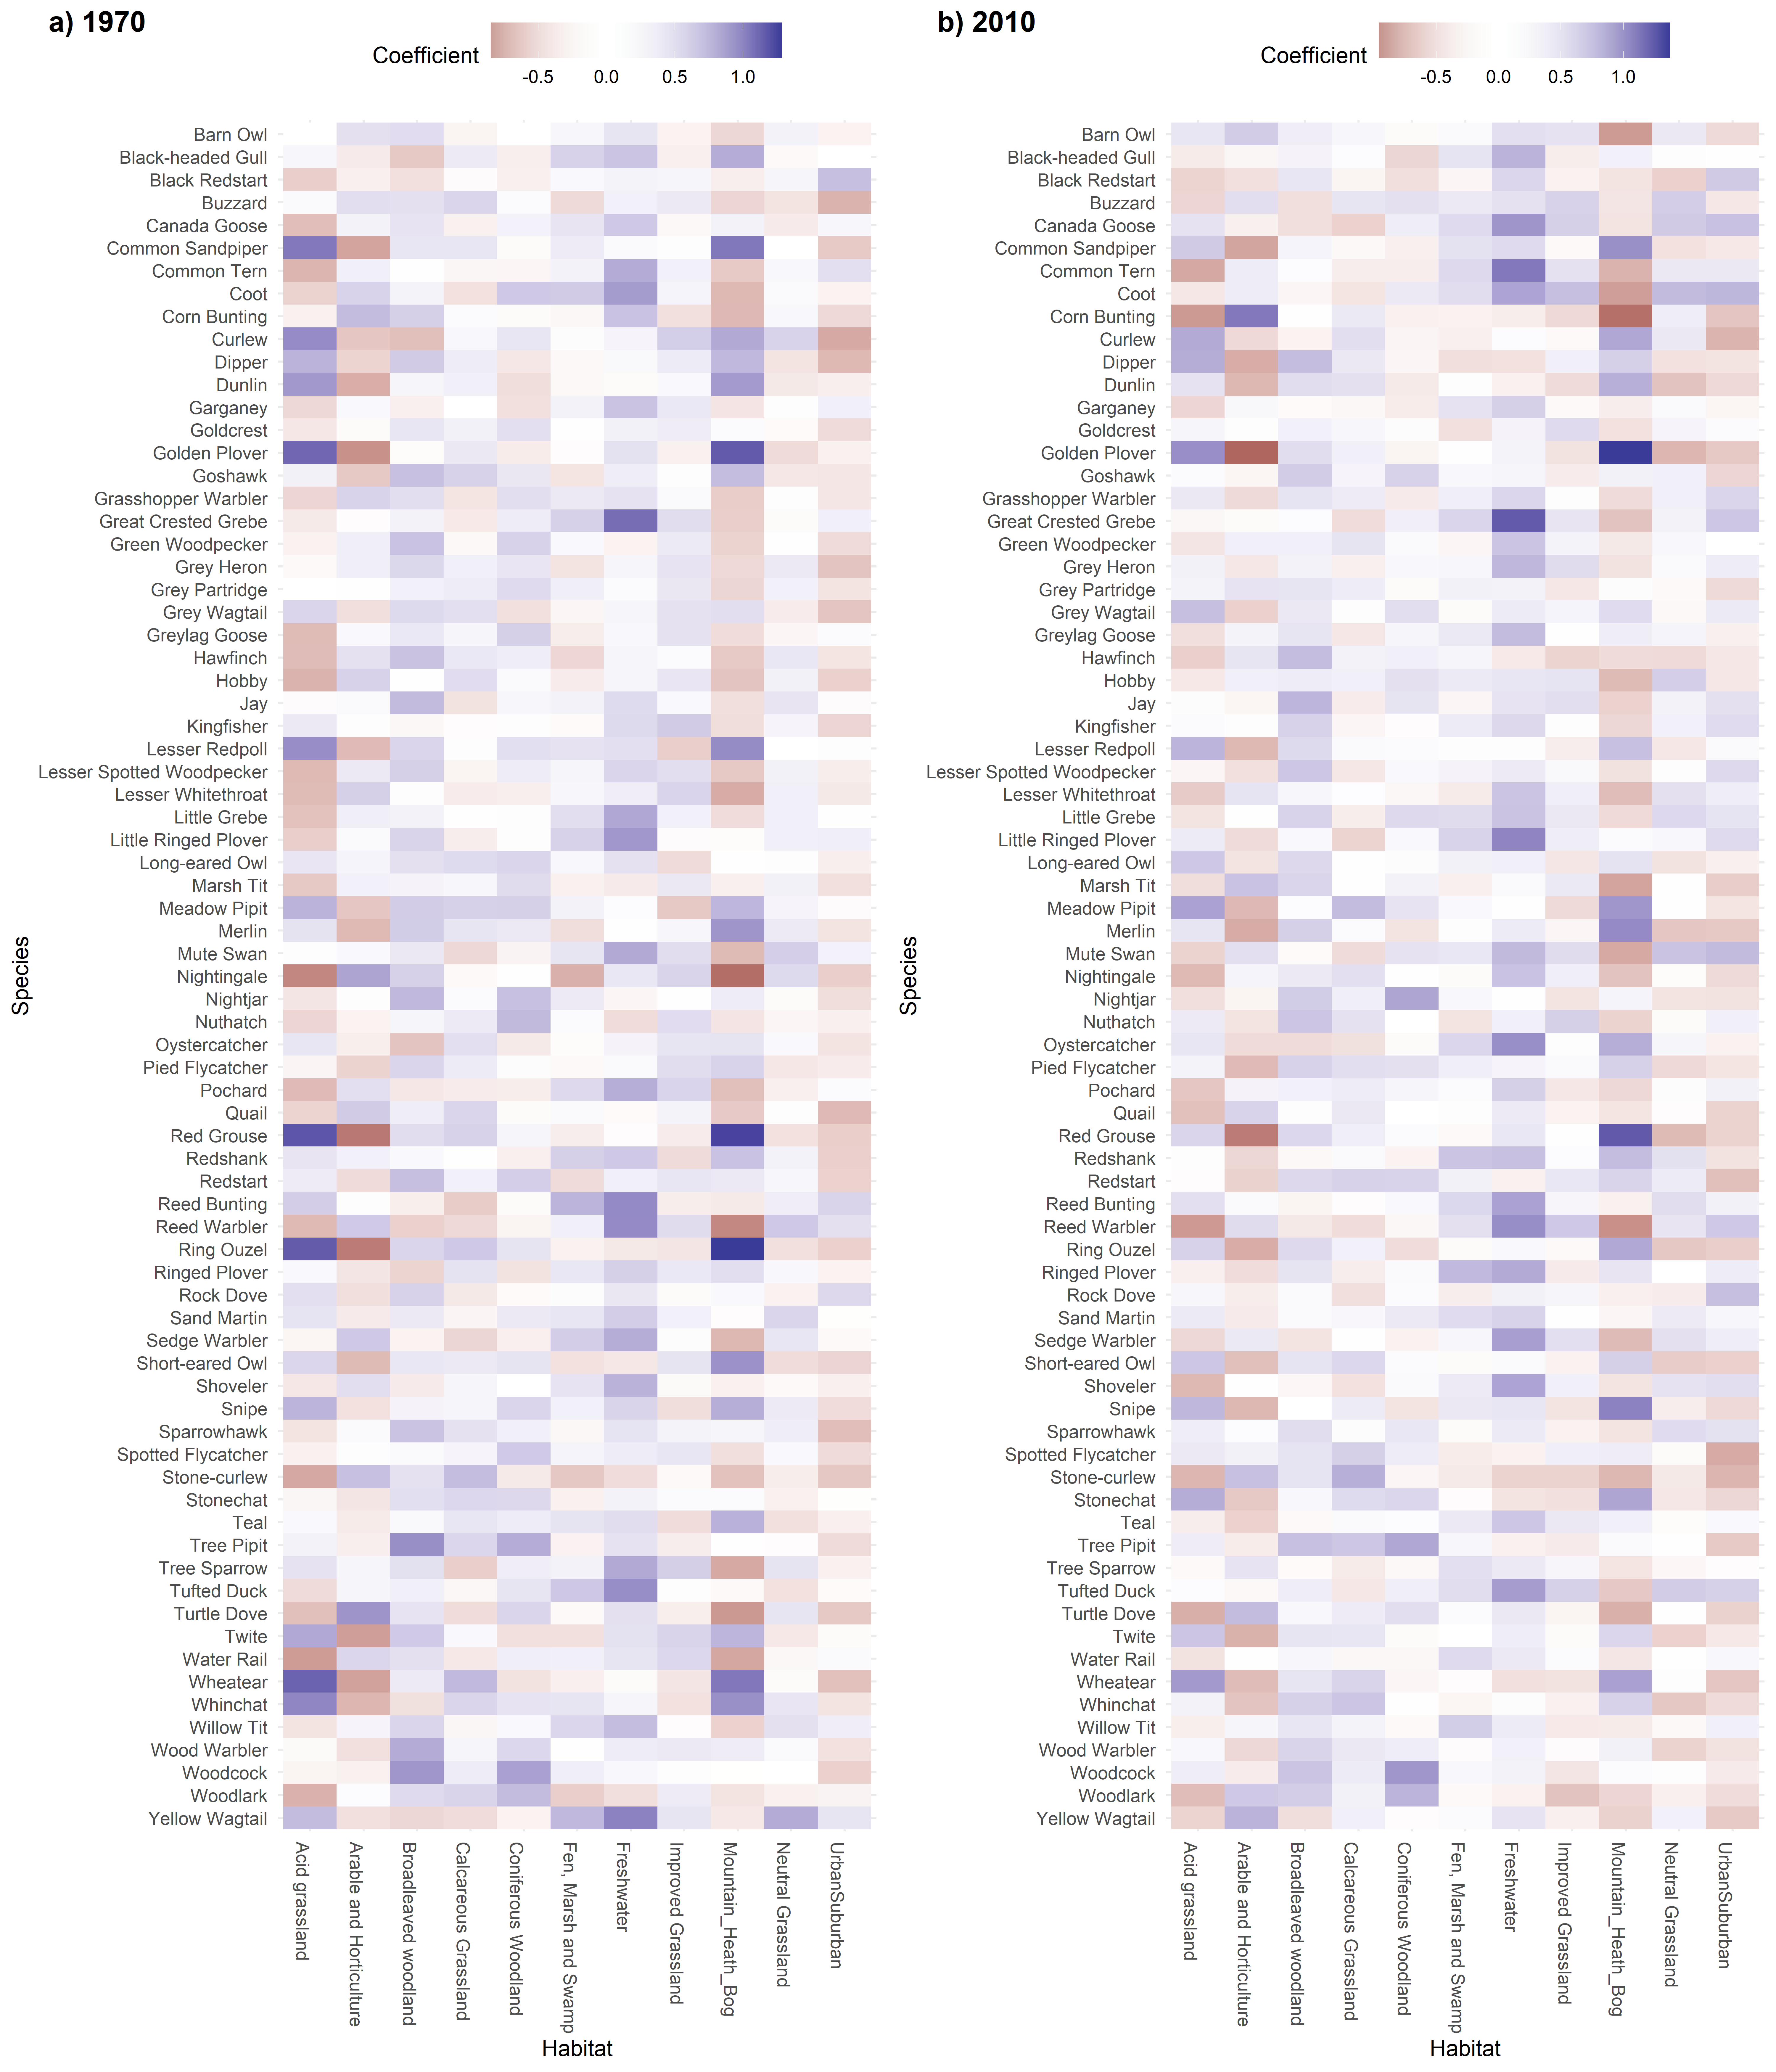
\includegraphics[width=\textwidth,height=0.7\textheight]{BirdMarkdowns/BirdImages/BirdHabitatbothHQ.png}
\caption{Fitted species-level environmental coefficients for breeding
bird dataset (excluding `possible' records)}
\end{figure}

\hypertarget{species-codistribution}{%
\subsection{Species Codistribution}\label{species-codistribution}}

\begin{figure}
\centering
\includegraphics[width=\textwidth,height=0.7\textheight]{BirdMarkdowns/BirdImages/SpecAssoc_1970_HQ.png}
\caption{Fitted residual species-association matrix (correlations) for
1970 breeding bird dataset (excluding `possible' records.)}
\end{figure}

\begin{figure}
\centering
\includegraphics[width=\textwidth,height=0.7\textheight]{BirdMarkdowns/BirdImages/SpecAssoc_2010_HQ.png}
\caption{Fitted residual species-association matrix (correlations) for
2010 breeding bird dataset (excluding `possible' records.)}
\end{figure}

\hypertarget{mcmc-convergence}{%
\subsection{MCMC Convergence}\label{mcmc-convergence}}

\begin{figure}
\centering
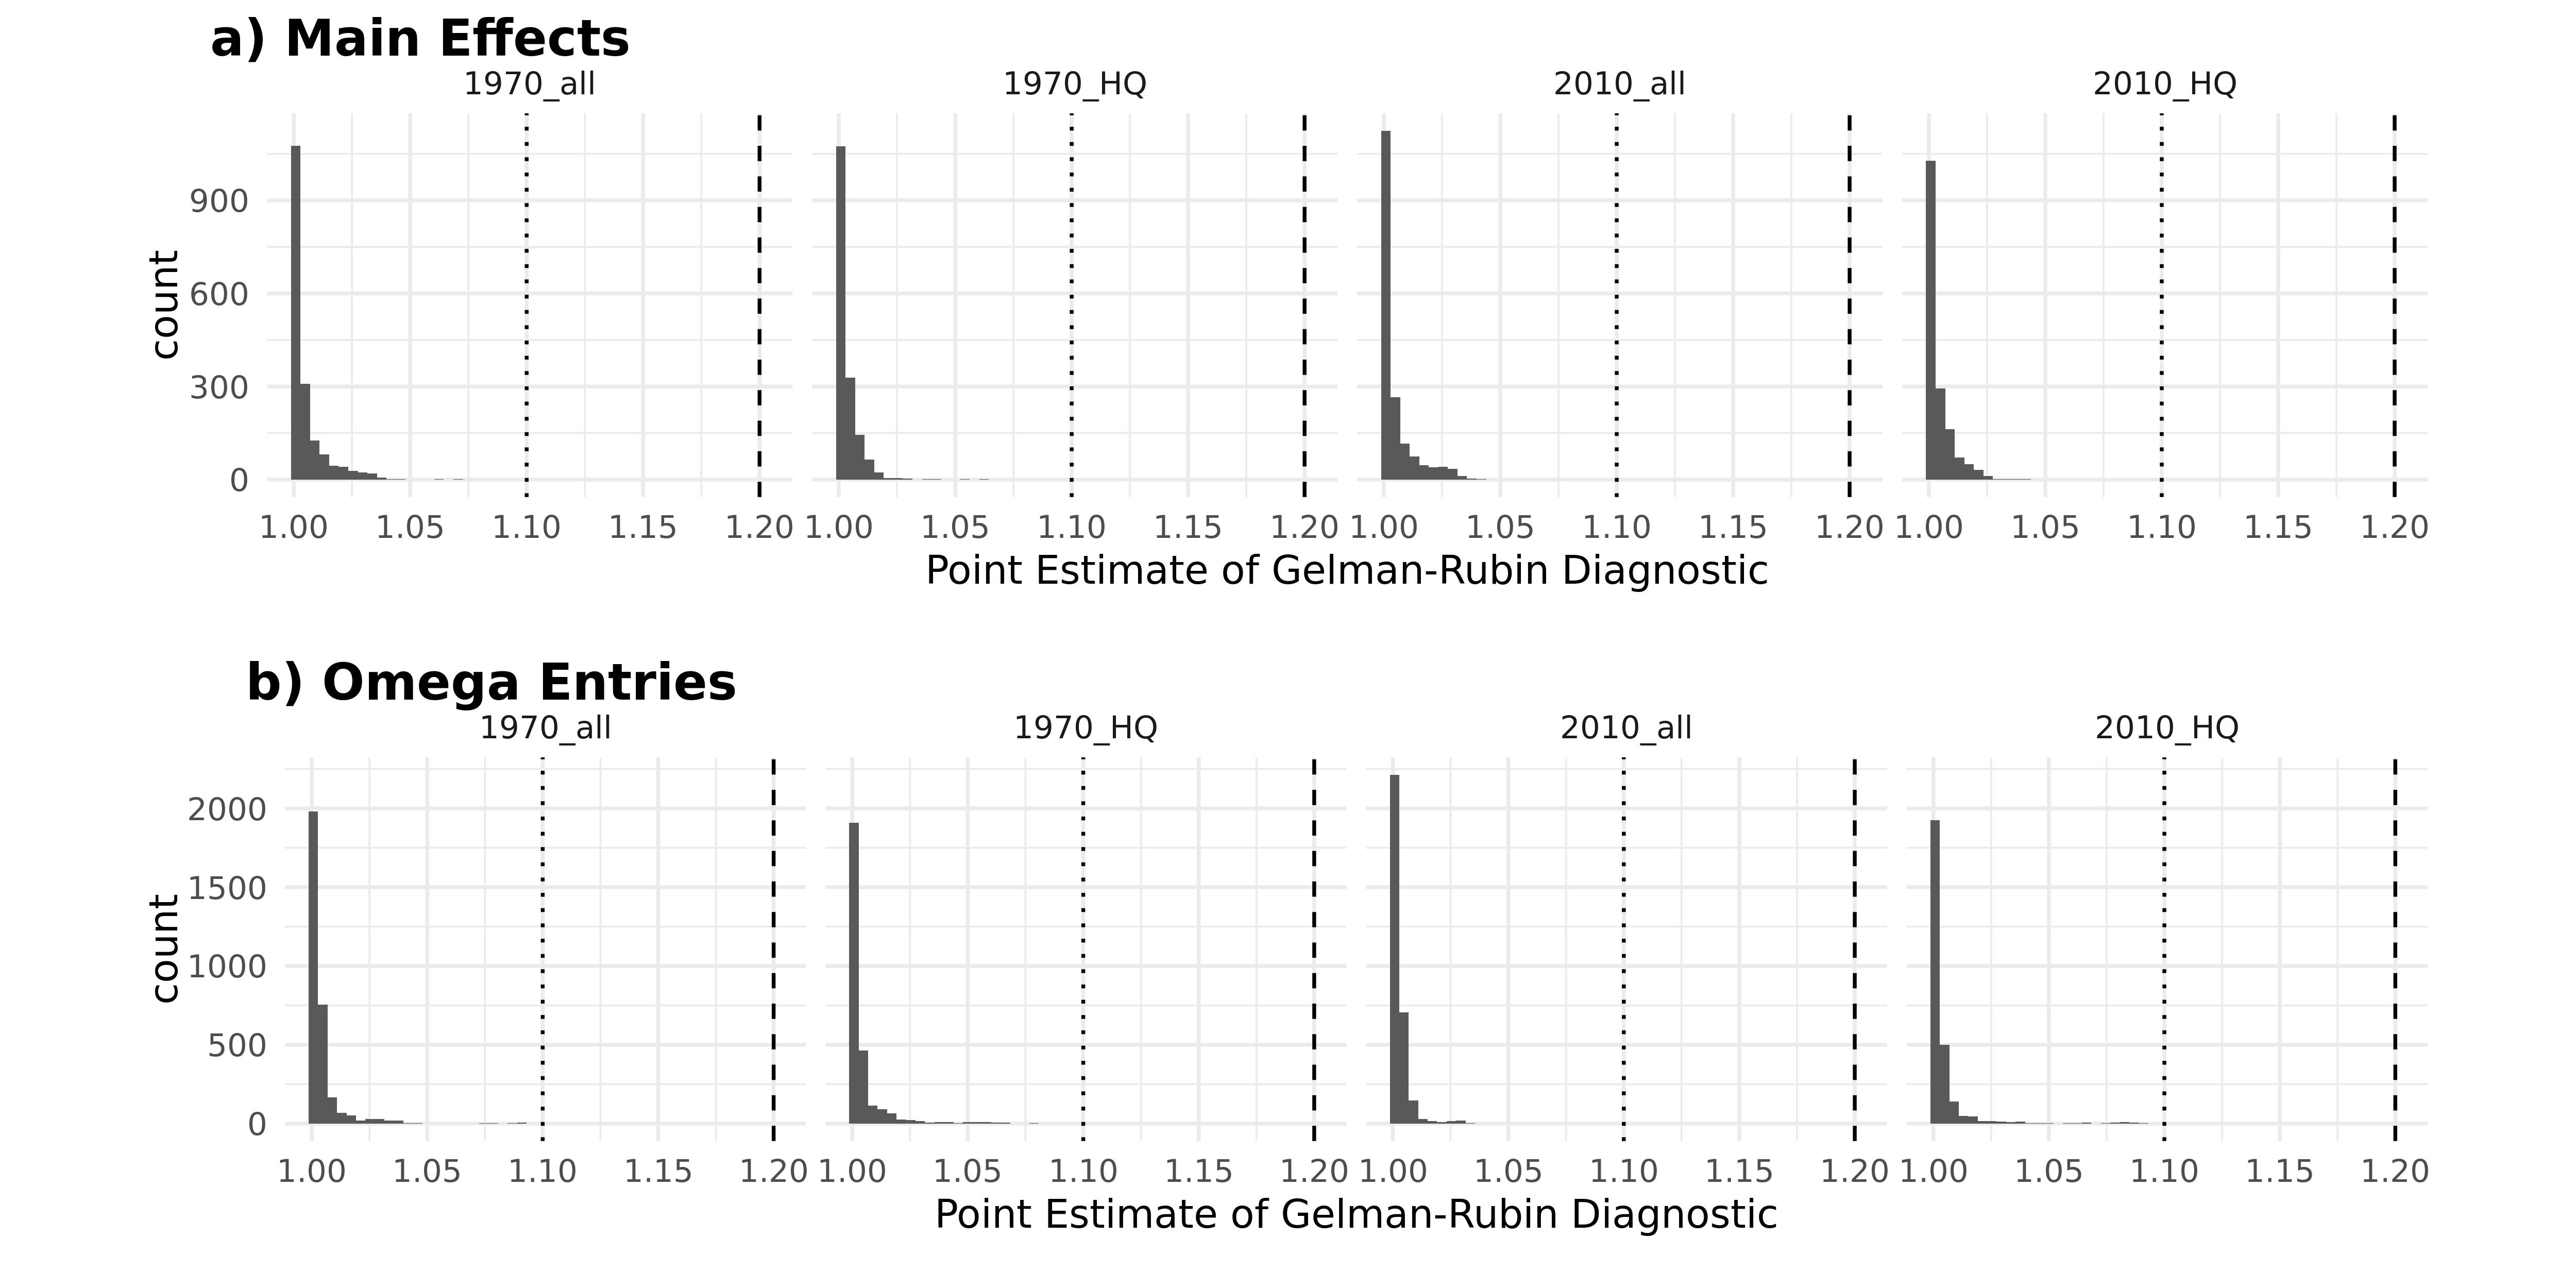
\includegraphics{BirdMarkdowns/BirdImages/ModelCovergence.png}
\caption{Distribution of Gelman-Rubin MCMC convergence diagnostic value
point estimates for the bird datasets, calculated from 4 independent
MCMC chains of the `full' model. Values are faceted by year and whether
all data is used, or excluding `possible' observations (HQ). a) Main
effect coefficients (i.e.~environmental and spatial variables). Largest
value was 1.069. b) Elements of the correlation matrix (\(\Omega\)).
Largest value was 1.102. All were well below the standard thresholds
indicating convergence is likely achieved.}
\end{figure}

\end{document}
